\chapter{Overview of the anonymous communication networks }
\label{chap:Overview}

This chapter reviews the history and evolution of Anonymous Communication Networks (ACNs), highlighting key milestones, technical developments, and influential systems that have shaped the field. The aim here is to provide the necessary background and context for understanding how modern ACNs have developed, what problems they were designed to solve, and why specific technical solutions were introduced. By presenting the main network families along with notable systems built on these designs, this chapter sets the foundation for all later analysis.

This overview is intended not only to familiarise the reader with the essential concepts and terminology, but also to clarify the motivation behind each architectural choice. Ultimately, this chapter serves as a reference point for the rest of the thesis, making it possible to understand the specific technical solutions that will be compared in detail later in the thesis.

The chapter begins with a historical overview, then presents the main technical approaches: single-hop proxies, Mix-nets, DC-nets, anonymous publication systems, onion routing, each with description of representative systems and their technical solutions. The chapter concludes with a classification and summary.

\section{History of ACNs}
The first paper that described the idea of ACN is considered David Chaum's master's thesis on Mix networks \cite{Chaum81}, written in 1979, published in 1981. To this day, most of the anonymous communication systems utilise ideas that were first described by Chaum. The Mix-nets design was ahead of its times, not only in terms of demand for anonymous communication, but also in terms of the computational power needed to repeatedly perform complex public-key cryptographic operations. It took more than a decade for the first anonymous communication networks to be successfully deployed.

The first ACN solutions were remailers, proxy servers that received messages and passed them accordingly to the instructions that were attached to the message.
The first widely used ACN-like solution was the Penet remailer \cite{penet}, deployed in 1993. However, it did not yet utilise Chaum’s concept; it was a simple single-hop pseudonymous remailer, also known as a Type 0 remailer, and did not ensure anonymity by design. It served as a proxy that stripped metadata from the message and forwarded it to the recipient, allowing for replies. The Penet had several security flaws, including the lack of encryption and the logging of user activity, and was eventually discontinued.

Around the same time, although initially less known, the Cypherpunk remailer was introduced, otherwise known as a Type I remailer. It was associated with the Cypherpunk movement, a movement that, since the late 1980s, promoted cryptography and privacy for everyone, rather than limiting them to military use, as had previously been the case. It placed strong emphasis on encryption and lack of logging, and enabled users to chain their messages through multiple servers. It was the first real-life implementation of Chaum’s concepts, although only partially.

Another important implementation was Mixmaster, also known as a Type II remailer, created around 1995. It implemented the most important Mix-nets concepts: layered encryption, batching, and mixing, and gained significant recognition. Over the years, many Mix network-based solutions have been introduced, addressing issues related to the previous designs.

Mix-nets are not the only design that was proposed. In 1988 David Chaum published a paper about DC-nets \cite{dc-nets} - an alternative approach for achieving anonymity for both sender and receiver. Similarly to Mix-nets, it provided a foundation for further research, and many later designs based their principles of operation on DC-nets. Even though there have been attempts of deploying ACNs based on DC-nets, none of the ACNs used today utilise this approach due to several limitations.

Another breakthrough design was onion routing \cite{onion-routing98, onion-routing-internet99}, a low-latency, connection-based, bidirectional communication network that, similar to the Mix-nets, utilises layered encryption. The work on it began in 1995 and was funded by the ONR, the science and technology agency for the U.S. Navy. The first paper on onion routing was published in 1996; however, the final version was published in 1997, and a year later it appeared in the \textit{IEEE Journal on Selected Areas in Communications}. Most ACNs used today are based on onion routing architecture.

One of the examples is Tor - the most popular ACN today, first deployed in 2002 as a direct successor to the original onion routing idea that was meant to be used by common people. The design was described in the 2004 paper \cite{tor-design}. During the years, it evolved and introduced many new features that can be seen today.
Another prominent project that is based on a slightly modified onion routing is I2P - the modification is named Garlic Routing. I2P is a peer-to-peer network, and every user also acts as a router. Theoretically, the work on I2P started in 2001; however, the architecture was completely redesigned in 2003. Similarly to Tor, it is constantly evolving.

One of the newer onion routing-based ACNs that can be used today is Lokinet, first described in 2018 \cite{loki}. Lokinet implements a custom protocol called LLARP, which is a low latency Anonymous Routing Protocol, and, contrary to Tor and I2P, it is placed on the network layer and can support any IP-based protocol.

Although onion routing dominated the scene of ACNs, they have some drawbacks, particularly vulnerability for traffic analysis. Even though Mix-nets are more resistant to this kind of attack, they suffer from significant latency. Loopix, proposed by Piotrowska et al. in 2017 \cite{loopix}, is an acceptable latency Mix-net architecture that led to a new rise in research on Mix-nets. One of the results of this increase is the Nym network \cite{nym}, first described in 2021. The official launch of NymVPN, a service that allows the utilisation of the Nym network, was carried out in early 2025.

\section{Single-hop proxies}
The principle of operation of single-hop proxies is straightforward: strip the metadata related to the sender before forwarding it to the recipient. The major advantage of them is their low latency due to simplicity and the fact that there is only one node between the sender and the receiver. However, such a single point of failure is not a desirable characteristic of an anonymous system, regardless of the claims of not keeping sensitive user data, as it imposes anonymity by policy rather than anonymity by design. As this architecture does not provide the anonymity by design property, it will not be treated as a proper anonymous communication network, however, due to its historical meaning it is mentioned here.

Notable examples from this category include Penet \cite{penet} and Anonymizer \cite{anonymizer}. In addition, many VPN services commonly used today can also be considered examples of this category.

\subsection{Penet}
Penet was the first widely known single-hop proxy and the most prominent example of the family of pseudonym-based solutions, called pseudonymous remailers or nym servers. Sometimes, they are also referred to as Type 0 remailers. Their common characteristic is that they remove sender-specific information that could potentially identify senders, assign them a pseudonym, and forward the message to the recipient with the possibility of reply. Penet was created in 1993 by Johan "Julf" Helsingius from Finland. The creation was a result of a discussion on a Finnish Usenet newsgroup about whether people should be required to use their real information for online communication. Johan believed that if such accountability were enforced on Internet users, they would find a way around it. To prove his point, he created Penet.

Remailers serve as an intermediary between sender and receiver. Penet, which served as such a remailer, removed metadata that could potentially identify the sender and then forwarded the message without sensitive data to the receiver. It also served as an e-mail box that allowed users to assign their pseudonymous identities to their messages and receive messages sent to their anonymous addresses.

Penet had some vulnerabilities that could potentially compromise its users. For example, it sends the messages in plaintext. The lack of confidentiality of these messages could have led to the disclosure of sensitive information in the presence of an eavesdropper. Penet also kept a list of its users with their real email addresses and its mapping to the anonymous ones. It posed a threat in case of breaking into the server.
Penet was closed due to legal issues in 1996.

\section{Mix-nets}

The first system that provided anonymity by design was described by David L. Chaum in his master's degree thesis, "Untraceable Electronic Mail, Return Addresses, and Digital Pseudonyms" in February 1979. Mix networks use public-key cryptography to hide both the sender and receiver of an electronic mail, as well as the content of their communication. They do it by encrypting a message with multiple layers of public key encryption and passing them through multiple nodes called mixes. Each node changes the message order, delays them, adds random information and padding in order to minimise the risk of traffic analysis and associating the sender with a given message; in other words, to obfuscate correlation between the input and the output. It also removes the corresponding layer of encryption and passes it on to the next node on the path. The simplified Mix-net architecture is presented in Figure~\ref{fig:mixnet}; each mix within the Mix-net decrypts a message that was previously encrypted with its public key, permutes the messages, and then forwards them to the next node or the final destination.

\begin{figure}[ht]
  \centering
  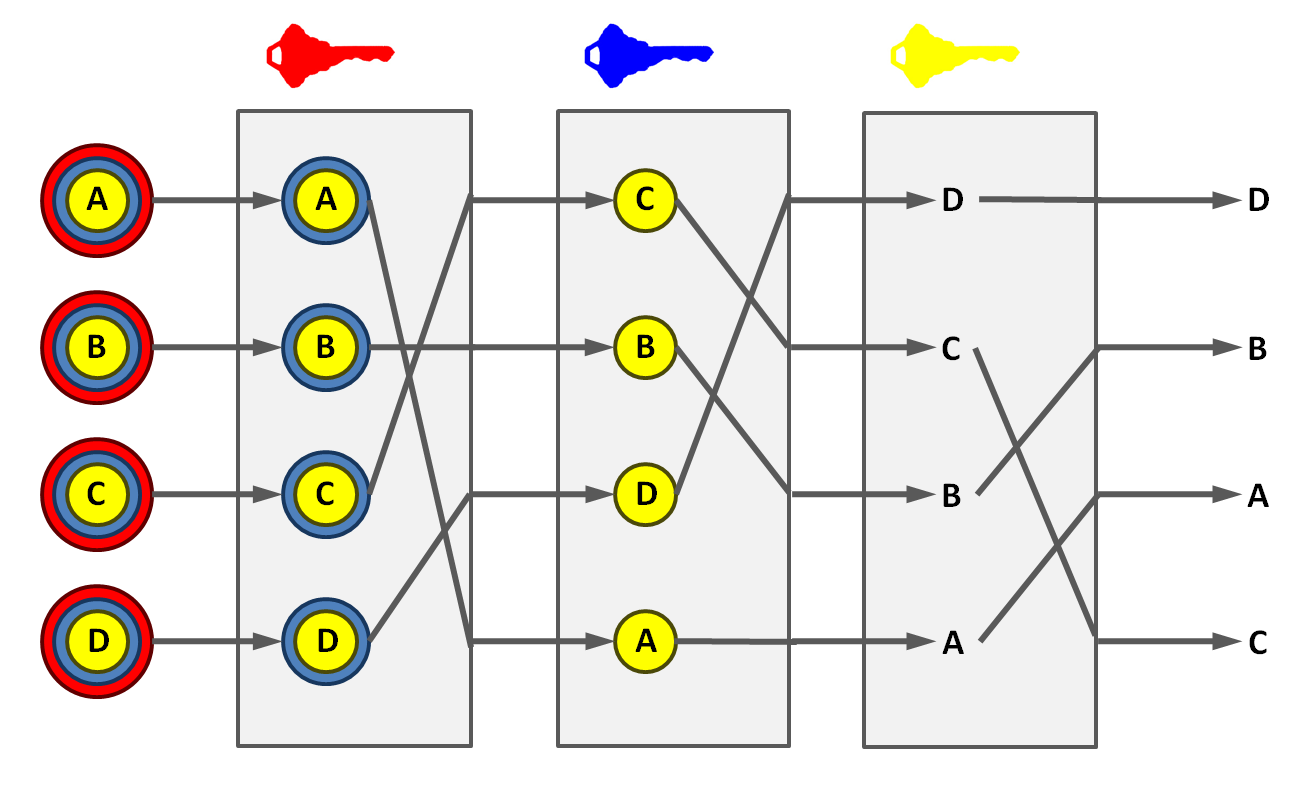
\includegraphics[width=0.7\linewidth]{Images/mix-net.png}
  \caption{Simplified Mix-net architecture. By Primepq, Wikimedia Commons~\cite{primepq_mixnet_2008}, licensed under CC BY-SA 3.0.}
  \label{fig:mixnet}
\end{figure}

In essence, it can be said that the sender knows all nodes in the path, each node knows only its neighbours, and the receiver knows only the final (exit) node. So, the identity of the recipient is only known to him, the sender, and the exit node; and the identity of the sender is only known to the first (entry) node.
The sender can send his message anonymously while the recipient can respond to the untraceable return address constructed using a real address, two random strings, and public-key cryptography. Communication participants exchange these addresses through multiple nodes, but only the addressee can decrypt them.

In 1964 \cite{Baran1964} Paul Baran, a Polish Jewish American engineer, proposed a solution to the traffic analysis problem; the downside of this solution was that it required a trusted common authority. Chaum's Mix-net network does not need a trusted third party to achieve resilience to traffic analysis. 

Mix-nets also propose digital pseudonyms in order to identify entities online. They are nothing more than public keys that can be used for signature verifications performed by an anonymous entity. The authority creates a list of pseudonyms and can decide which are trustworthy and which are not. The pseudonyms contained in a letter from each entity to the authority are processed together in a single batch and create together a complete roster. These letters can also be protected to provide an additional level of security. A person cannot be traced by his pseudonym in the final list; therefore, it allows verifying and communicating securely with assured anonymity. 

One of the major disadvantages of the Mix-net is high latency correlated with public key cryptography, delays, and other aspects that are supposed to provide anonymity; therefore, anonymity for more latency-sensitive purposes must use other solutions.

\subsection{Early related designs}
Various anonymous communication systems utilised concepts from the original Mix-nets design, introducing certain modifications in order to address certain aspects of anonymous communication.
Many of these systems were associated with large latencies associated with the Mix-nets architecture that made it impossible to use them in more time-sensitive scenarios such as web browsing.

For these systems, it can be mentioned, among others, Babel, an anonymous remailer described in 1996 \cite{babel}, which aimed to quantify the dimensions of anonymity, provide a way of measuring it and enhance the security of the network. Another example was a paper about Stop-And-Go MIXes (SG-MIXes) \cite{stop-and-go} that introduced random delays in order to be more resilient to traffic analysis and remove the requirement of collecting a fixed-size batch of messages.
ISDN-MIXes \cite{Pfitzmann91} is another Mix-net-based design from 1991 for untraceable communication for services such as telephony. One of its major advantages is the very small bandwidth overhead.

The first Mix-net-based solutions that were successfully implemented and gained significant recognition were anonymous remailers.
In 2000, the Web MIXes system \cite{web-mixes} was proposed as one of the first described solutions for Internet browsing using Mix-nets. The project was successfully implemented and gained recognition.
After initial Mix-net designs, where mixes were treated as specific servers to whom clients connect, propositions to make peer-to-peer designs occurred where each user also relayed traffic for others, acting as a mix in the network. Within this category, there are solutions such as MorphMix \cite{morphmix} or Tarzan \cite{tarzan}.

\subsection{Anonymous remailers}
Anonymous remailers were the first real-life implementations of Chaum's ideas that gained significant recognition. There are three types of anonymous remailers, or four, if pseudonymous remailers that were described before are counted.

\subsubsection{Cypherpunks remailers}
The first anonymous remailers, also known as Type I remailers, were initially created by the Cypherpunk movement. Cypherpunk remailers can only be used for one-way communication, as there is no possibility for the recipient of the message to reply. 

Cypherpunk remailers, as the whole Cypherpunk movement, attaches huge importance to the cryptographic aspect of communication; therefore, messages were encrypted in order to provide confidentiality, usually with the software from the PGP family.

Another important concept introduced with Type I remailers was chaining, which means that instead of one remailer that will be more than intermediate in the connection between the sender and the receiver, eliminate the single point of failure issue and increase the anonymity of the sender, since the second and every next remailer in the path does not know anything about the sender’s identity and the first remailer does not need to know the identity of the sender.

Contrary to the Penet remailer, Type I remailers do not keep a list of users or any activity logs.
One of the greatest weaknesses of cypherpunk remailers is their vulnerability to traffic analysis, and therefore to correlating messages with the sender by the order of them.

Cypherpunk remailers gave the foundation for other types of anonymous remailers.

\subsubsection{Mixmaster}
Mixmaster, also known as Type II remailer, is another type of anonymous remailer that, similarly to Type I, allows for one-way anonymous communication, unless, of course, the sender himself includes a reply address in the message itself. It was created by Lance Cottrell around 1995 and later maintained by Len Sassaman and Peter Palfrader. Mixmaster operates on fixed-size packets, and one of the greatest improvements in comparison to the Type I remailer is message reordering (mixing) that prevents the possibility of traffic analysis. Mixmaster sends messages through intermediary nodes via the SMTP protocol.

\subsubsection{Mixminion}
Mixminion, also known as Type III remailer, further addresses the issues related to its predecessors. Similarly to Type II remailers, it uses fixed-size packets that are reordered and forwarded with appropriate encryption through a chain of servers called mixes with their public keys. A single mix cannot correlate the sender with the recipient. 

In order to reply to messages, Mixminion uses single-use reply blocks, also called SURBs, that are a way of anonymous responses. They are hidden partial paths included in the message that give the possibility of responding without revealing the sender’s identity. Each mix in the chain can unwrap its layer and encrypt the message.

The initial release of Mixminion was in December 2002, and one year later the paper describing the design was published \cite{mixminion}.

\subsection{JAP}
JAP is an anonymous communication network known by many names: Web MIXes, Java Anon Proxy, JAP, JonDonym, JonDo. Despite the naming confusion, all of them refer to a proxy system designed to provide anonymity on the Web. The system was first described in 2000 in a paper "Web MIXes: A system for anonymous and unobservable Internet access" \cite{web-mixes}. Later, the project was deployed as part of the AN.ON project of the Technische Universität Dresden, the Universität Regensburg, and Privacy Commissioner of the state of Schleswig-Holstein under the name Java Anon Proxy (JAP), which was directly taken from one of the system components. In 2007, the project diverged into for-profit JonDonym (AN.ON substitute), and the proxy itself got the name JonDo (JAP substitute), and the entity responsible for the commercial branch development was JonDos GmbH. Regardless of these administrative and name changes, the system will be treated as one within this paper. It initially supported only HTTP and HTTPS traffic, although it was later expanded for other protocols, and had several interesting technical solutions that made it suitable for web browsing even though it utilised the high-latency architecture of Mix-nets.

Key components of the WebMIXes include: 
\begin{itemize}
    \item Java Anon Proxy client
    \item MIXes cascades
    \item Cache Proxy
    \item Information Service
\end{itemize}

\textbf{Java Anon Proxy client} is the client software written in Java in order to achieve platform independence. It connects to the first MIX of the MIX network through the Internet. It periodically sets up dedicated bidirectional channels for data transfer. If a user wants to send a message it is first transformed into the MIX-format and passed through the MIX cascade. If a user wants to send a smaller message than a given size, it is padded to avoid volume correlation. On the other hand, if he wants to send a large message or streaming data, the message is split into several time-slices and it is sent slice by slice with an appropriate Slice ID (SI). The idea of slicing was first introduced in the previously mentioned ISDN-MIXes. If there is nothing to send by a given client, a dummy message is sent. An adversary that wants to correlate a message with the specific sender is unable to do so as with equal probability it can be any of the active clients in a given moment and he is unable to tell the difference between the real message slice and a dummy message as they are both encrypted. As the channels are bidirectional, it is also responsible for handling the responses. Messages that are sent via JAP are also filtered in respect of potentially compromising content like cookies and JavaScript. On top of that JAP also utilises Information Service (info-service) in order to measure anonymity. Each user has limited bandwidth and the number of concurrently used time slices. Each time he wants to send a slice he has to provide a ticket. The ticket-based authentication system uses the blind signature algorithm invented by David Chaum \cite{blind-signatures} in order to preserve users' privacy. This authentication mechanism aims to prevent flooding and DoS attacks.

\textbf{MIXes cascades} are dedicated servers connected with each other through the Internet, although authors in the paper suggest that ideally they should be connected with dedicated high-speed connections instead, however it would be too complex and expensive. The chain of MIXes that mediates between the sender and the receiver is called MIX-cascade. Similarly to the original Mix-net design each MIX node strips a layer of encryption, creates a batch of messages and reorders the messages and forwards the data to the next MIX. The last one in the cascade sends it to the cache-proxy. MIXes, similarly to JAP, also send dummy traffic to each other.

\textbf{Cache Proxy} is an element responsible for sending the data from the last MIX to a specific web server that the user requested. It sends back the response through the same bidirectional channel, although in a reverse order. It also loads all objects embedded into the requested HTML page. This idea was first introduced in the Crowds project. Moreover, as the name suggests, it is responsible for caching the responses which helps to reduce the number of calls to the Internet.

\textbf{Information Service} is a service providing information about MIXes’ addresses and public keys, current traffic and MIXes availability and the provided level of anonymity which is calculated by taking into account the number of currently active users which is directly associated with the possibility of the intersection attack. Each user can set a threshold of anonymity he wishes to maintain and once the level falls below that threshold he will be warned.

The WebMIXes project underlined the importance of the usability perspective and ease of configuration and use, as well as the portability of the JAP software so that it could have been run on as many diverse devices as possible. It also provides a built-in integration with web proxies that helps to work behind restrictive proxies, firewalls, et cetera. in order to provide better accessibility.

In JonDonym users also had the possibility of choosing Mix Cascades in order to avoid organisations that they do not trust. In the past, it used to be one of the more recognised ACNs, although as it is not functioning today, it cannot be considered within the comparative analysis.

\subsection{Design considerations}

During the evolution of Mix-nets, several important design considerations emerged, including the development of different mixing and batching strategies, message formats, and network topologies. These aspects played a crucial role in shaping the functionality and security of modern Mix-nets.

\subsubsection{Mixing and batching strategies}
Several mixing and batching strategies were introduced in various papers and projects. One of the first attempts to provide a formal framework for modelling mixing networks based on the mixing and batching strategy was proposed in 2003 \cite{generalising}. It was based on the 2002 paper \cite{mix-attacks} in which certain types of mix networks were distinguished and categorised along with attacks on them. Those strategies included:
\begin{itemize}
    \item threshold mix
    \item timed mix
    \item threshold or timed mix
    \item threshold and timed mix
    \item threshold pool mix
    \item timed pool mix
    \item timed dynamic-pool mix (Cottrell Mix)
\end{itemize}

\textbf{Threshold mix} is a strategy where the mix collects a certain numbers of messages and then forwards them. In \textbf{timed mix} mixes forwards messages after a specific time period. With \textbf{threshold or timed mix}, the mix either collects a certain numbers of messages and then forwards them or forwards messages after a specific time period. In case of \textbf{threshold and timed mix} the mix collects a certain numbers of messages and forwards them after a specific time period. In \textbf{threshold pool mix} when $n+f$ messages accumulate in the mix, where n is a threshold and f is a pool size, n randomly chosen messages are forwarded while f messages are kept in the pool for the next iteration. In \textbf{timed pool mix} every specific period of time messages are sent, however a fixed number of random messages (a pool) are kept in the mix. Lastly,  
\textbf{timed dynamic-pool mix (Cottrell Mix)} is similar to the timed pool mix combined with threshold pool mix, however only the certain fraction of messages surplus, after the pool subtraction, are forwarded every specific period of time.

\subsubsection{Message format}
Over the years, specific message formats for Mix-nets have been proposed to improve security, for example, by hiding metadata and routing information that helps break the linkability between incoming and outgoing messages or protecting against attacks such as the tagging attack where the attacker modifies messages by embedding tags that he wants to detect in other parts of the network in order to get routing information. Minx \cite{minx} was one of the first propositions to address these issues. The format uses RSA for the standard Mix-net encryption along with anonymous reply blocks, AES with IGE mode that helps to detect message manipulation, and, as the IGE mode propagates errors, destroys the modified message by changing the content into garbage. At the same time, the format imposed a low computational and communication overhead. Minx has a vulnerability that was discovered in a 2008 paper \cite{fix-minx}. The paper, besides describing the vulnerability and a chosen ciphertext attack that exploits it, provides a fix for the Minx format that would address this issue by replacing explicit session key and next hop header fields by utilising hash functions.

Yet another message format, Sphinx, was proposed in 2009 \cite{sphinx}. The goal was to provide the most compact and yet fully secure scheme. Sphinx addressed issues of the Minx design while keeping all the desirable properties of it. One of the changes was using ElGamal instead of RSA. Sphinx also includes replay protection and formal proofs of security, which Minx lacked.

\subsubsection{Topologies}
There are several possible topologies in the Mix-nets that appeared throughout the years. These topologies were distinguished and analysed in terms of anonymity and overhead in 2010 \cite{topology}. The first topology that appeared in the original Chaum 1981 paper was a cascade topology in which the mixes create a simple path where each node is connected only with its predecessor and successor (excluding the first and last nodes). Due to the unlinkability property of Mix-nets, the cascade can be fixed, and there is no need of permutations of paths as in the onion routing that will be described later. The drawback of this topology is its poor scalability and availability, as each mix in the path is a potential point of failure and there is a high risk of bottlenecks. Instead of a single cascade, there is also a possibility of a topology where there are many cascades - it is called multi-cascade topology.

One of the alternate topologies is a fully connected network, where each node is connected to any other node in the network. It fixes the availability issue as there are many potential routes from one mix to the other. It does not fix the issue of scalability, as adding a new node implicates the necessity of adding a connection to every other node in the network. The drawback of this topology is the fact that messages cannot be freely mixed as there are several possible directions for a message from the node.

Another possible topology, mostly used in the latest Mix-nets, is a stratified topology. Each node is assigned to a certain layer and is connected to every other node from the previous layer and with every other node in the next layer; however, the direction of the messages in the network is fixed. With this topology, scalability and availability are improved, and all messages in the node can be mixed together regardless of their origin and destination, contrary to the free route design.

\subsection{Loopix}
The development of Mix-net-based systems continues to this day, although it is definitely less popular than onion routing-based solutions. One of the newer propositions in the MIX world is the Loopix system, proposed in the 2017 paper \cite{loopix}. It used ideas from Stop-and-Go MIXes, creating a simplified version of it called the Poisson mix. The messages do not use synchronous rounds, as with some different Mix-net designs; they are asynchronously and nondeterministically delayed using an exponential distribution. Messages arriving at a given entity within the network follow the Poisson distribution. As a solution for a smaller user base and increased security, cover traffic is introduced between entities in the network, including loop traffic. Loop traffic, whose concept is similar to the 2003 paper \cite{n-1}, where a user sends messages to himself, helps to detect active attacks and blocking of messages and, along with drop cover traffic, aims to hide communication patterns. Loopix provides a modifiable trade-off between anonymity and usability by changing message delays and the real to cover traffic ratio. Loopix uses providers to manage access and store offline messages. These are semi-trusted nodes that users connect through. The Loopix mixes create a stratified topology, which means that they are grouped in layers, and each node is connected to every node from the previous layer and every node from the next layer. When a user wants to send a message, he randomly chooses a node from each layer. The messages sent on the Loopix network follow the Sphinx format.

Loopix opened a new chapter in mix networks as it serves as a basis for other Mix-nets that are created to this day, Nym \cite{nym} being an example of such a network.

\subsection{Nym}
The Nym network was described in 2021 \cite{nym}. The network is based on the Mix-nets architecture and heavily utilises concepts from the Loopix network and can be considered an implementation of Loopix, enhanced with economic incentives. Mixes on the network are rewarded with NYM tokens using a mechanism called "proof of mixing". The tokens provide economic incentives which are not present in other volunteer-based networks and aim to encourage more people to host mix nodes. One of the main goals of the network is to introduce a global adversary-proof solution that is not present in solutions such as Tor. In addition to a decentralised Mix-net, Nym includes an anonymous credential cryptosystem.

Nym network architecture consists of the following elements:
\begin{itemize}
    \item mix nodes
    \item gateways
    \item service providers
    \item Nym blockchain
    \item nympool
    \item validators
\end{itemize}

\textbf{Mix nodes} are nodes that create a network called Mix-net that relays, decrypts its specific layer of encryption, reorders and delays messages asynchronously as in the Loopix network. \textbf{Gateways} are entry points for the Nym network. Users can choose whether they want to always use the same gateway or not. Similarly to the Loopix design, they are also able to store messages for users that are offline. \textbf{Service providers} are entities that provide certain services through the Nym network. They receive cover traffic that is indistinguishable from the real users’ traffic, which enhances users’ privacy. \textbf{Nym blockchain} is a decentralised blockchain structure, maintained by validators, that distributes network-wide information regarding public node reachability and public keys, configuration parameters and other publicly available data that is necessary for proper functioning of the Nym network. \textbf{Nympool} is a shared pool of funds supporting the Nym network. Periodically validators algorithmically distribute rewards from the nympool to the nodes (validators, gateways, mixes) and to the service providers that redeem users’ service credentials. \textbf{Validators} maintain the Nym blockchain, including nympool, as well as issue bandwidth and service credentials that prove the allowance of sending data through the Mix-net and the right to access a certain service, respectively.

The flow of users connecting to the service provider in the Nym network works as follows: A user deposits his NYM tokens, earned by operating a node, purchased or received from a service provider, in the nympool and obtains credentials with the help of the validators. These credentials cannot be directly linked to their use due to blind signatures. With the bandwidth credential, the user can access the gateway of his choice. The gateway validates the token on the Nym blockchain and submits a commitment of the credential to the validators in order to avoid double-spending. The user and the gateway establish a shared secret for data encryption and a pseudonym associated with the credential that allows for tracking bandwidth consumption as well as for offline storage. From now on, until the bandwidth credential expiration or consumption, the user can use the Nym Mix-net through the gateway. Although the gateway has knowledge of when the user is accessing the network, it is not aware of where his messages are sent. The message from the user is sent to the recipient’s gateway, from which the recipient can pull the messages. The recipient is either a service provider, a validator, or another user. If the recipient is a service provider that provides a paid service, a service credential is needed to access the service. The logic behind the handling of the service credentials is similar to that of the bandwidth credential.

\subsection{Other designs}
In recent years, other Mix-net designs have appeared.
Katzenpost \cite{katzenpost} being one such example, aims to fix certain issues associated with the Loopix design. It puts a great emphasis on implementing post-quantum cryptography algorithms into the mix network, as well as changing a point of failure in the form of a single service provider into scattered distribution across multiple providers, similarly to a distributed hash table form. The project is still in development. Recently, the design was described in the Echomix paper \cite{echomix}, where Katzenpost is defined as the Echomix implementation.

Besides Loopix-based designs, there are also unrelated recent approaches to the topic of Mix-nets, including Vuvuzela \cite{vuvuzela} that aimed to minimise metadata related to the communication process, Riffle \cite{riffle} that aimed to decrease bandwidth and computation costs for the sake of file sharing and microblogging, or cMix \cite{cmix} that reduces public key cryptography-related latency and the overhead for the client by utilising precomputation. The cMix uses a threshold and a timed mixing strategy, which may potentially still introduce significant latency, especially for small numbers of users. Moreover, fixed cascade topology suffers from the issues described in the topology subsection, for example, reduced availability. The paper suggests a multi-cascade approach as a potential answer for this issue.

\section{DC-nets}

DC-nets are anonymous communication networks based on the dining cryptographers problem described by David Chaum in his 1988 paper \cite{dc-nets}. Despite the name, the problem is not related to the dining philosophers problem. It considers the problem of secure multiparty computation of the boolean XOR function. 
The problem can be described as follows: assume that three cryptographers are dining together. The waiter informs them that their meal has already been paid for by someone but does not reveal the identity of the payer. It is assumed to be one of the dining cryptographers or the National Security Agency (NSA). In order to determine whether it was one of them who paid or the NSA, they have to perform a certain two-stage protocol.

In the first stage, every pair of cryptographers establishes a one-bit secret. For three dining cryptographers, there are three such secrets: AB, AC, BC.
In the second stage, each cryptographer who did not pay announces the result of an XOR operation on the secrets he shares with his two neighbours. On the other hand, if a certain cryptographer paid, he announces the opposite of this XOR operation.

After three announcements are revealed, it can be determined whether it was one of the cryptographers who paid or was it NSA. This can be done by performing another XOR operation on these three bits. If the result is one, it means that it was one of the cryptographers who paid for the meal. If the result is zero, it means that none of the cryptographers paid; therefore, the NSA paid.

Figure~\ref{fig:dining_cryptographers} illustrates two scenarios in the dining cryptographers protocol: the case in which none of the cryptographers pays for the meal, and the case in which cryptographer \textit{A} pays.

\begin{figure}[ht]
  \centering
  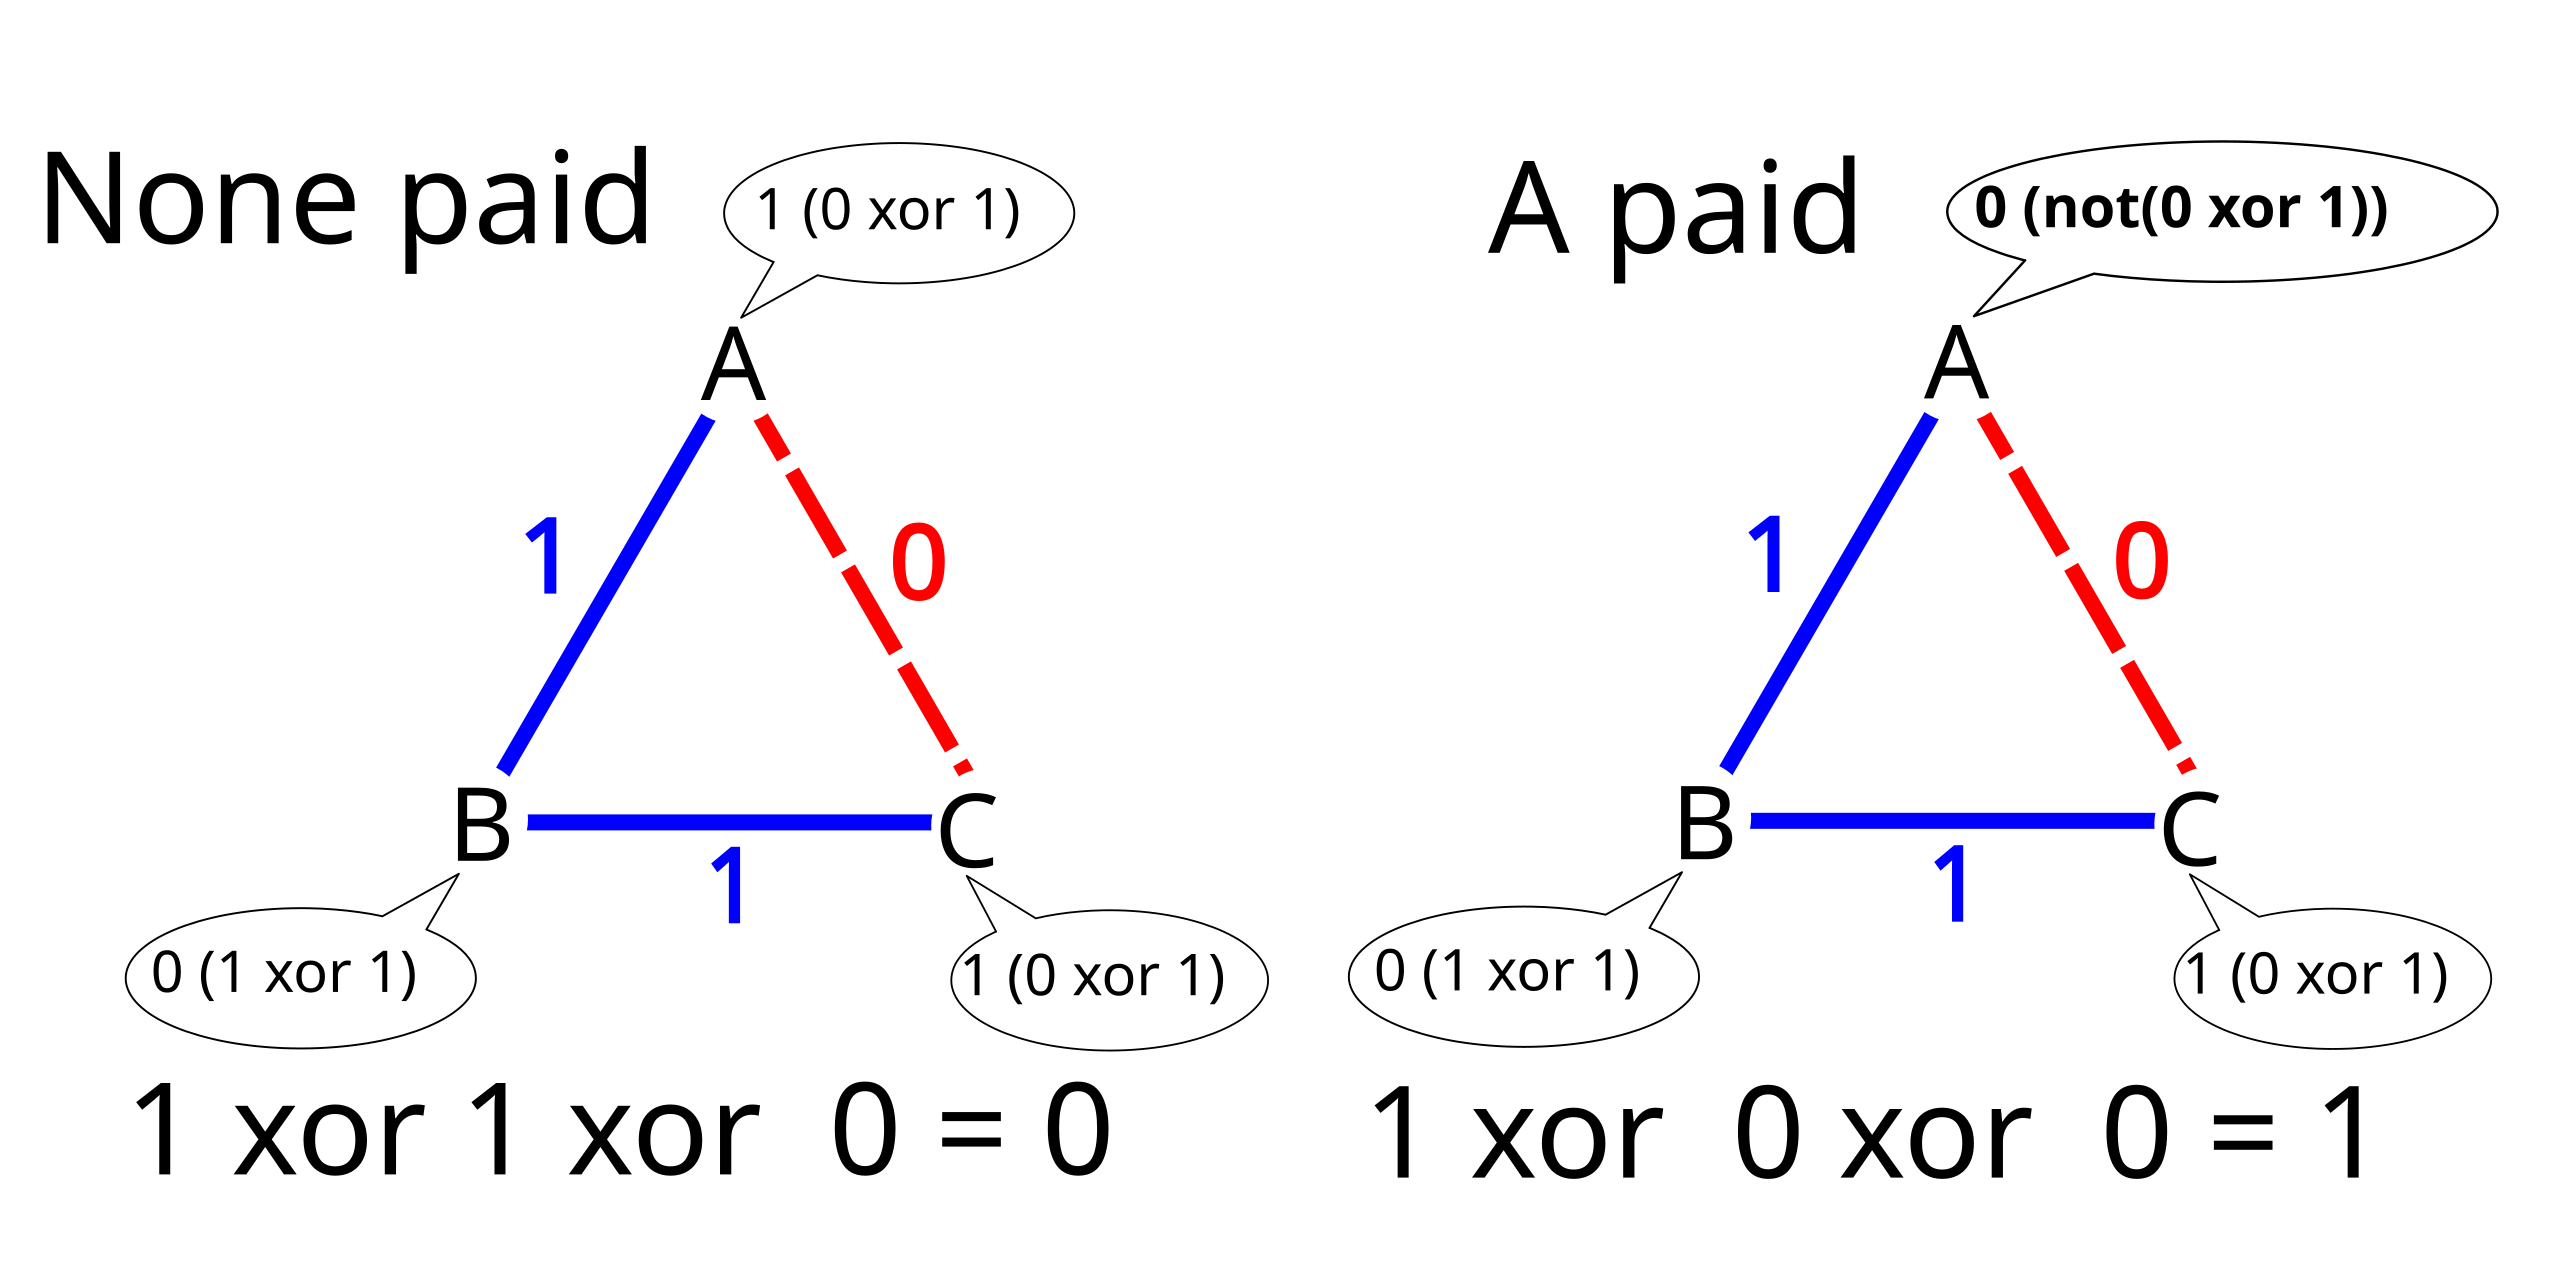
\includegraphics[width=0.7\linewidth]{Images/dc.png}
  \caption{Illustration of the dining cryptographers problem. By PauAmma, Wikimedia Commons~\cite{dining_cryptographers_pauamma}, licensed under CC BY‑SA 3.0}
  \label{fig:dining_cryptographers}
\end{figure}

There are several limitations to the dining cryptographers problem. Firstly, only one cryptographer can pay for the meal. Secondly, each cryptographer is trustworthy, meaning he always presents information that is true. Thirdly, each cryptographer must share a secret with every other participant, meaning that will be in total $n * (n-1) / 2$ connections, creating a complete graph.

The proposed protocol to solve the dining cryptographers problem can be easily converted to anonymous communication of longer messages. While sending messages bit-by-bit might be problematic, it can be replaced with fixed-size blocks, and the sender, instead of performing a negation of the XOR operation he performed on the secrets he shares with his neighbours, performs an XOR of these secrets with his message. The message is broadcasted by design; however, certain improvements can be made in order to provide confidentiality and authenticity - public-key cryptography can be utilised where each participant can have a public key associated with a pseudonym. The sender can include a digital signature in his message to prove the authenticity of the message. Moreover, in order to provide confidentiality (or secrecy), he can encrypt this message with the public key of the recipient he wants his message to be transferred to. Each network member will receive the encrypted message; however, only the recipient, the owner of the private key, will be able to decrypt it.

Chaum also proposes other potential improvements to the design, such as slot reservation.
The original DC-Nets design aimed to demonstrate the dining cryptographers problem and sketch potential implementations of them. However, they cannot be used in the original form in real use cases due to the issues associated with this simple design. Similarly to Chaum’s Mix-Nets, his DC-Nets introduced a new branch of ACNs, creating a basis for the future work of other researchers.

\subsection{Related designs}
Among systems or propositions based on DC networks, which similarly to Mix-net-based solutions were meant to address some issues of the original design, it is worth mentioning The Dining Cryptographers in the Disco protocol \cite{dc-disco} and CliqueNet \cite{clique-net}, a peer-to-peer, practical, self-organising, resilient, scalable, and anonymous communication network that was proposed in late 2001 and aimed at fighting surveillance from solutions like Carnivore \cite{carnivore}. CliqueNet evolved into the Herbivore \cite{herbivore} network; however, the goals remained mostly the same. Another example of DC-net-based design with efficiency improvements and multicast focus was described in the XOR-Trees paper \cite{xor-trees}. A notable paper on improvements to the DC-net design - among others in terms of jamming detection, efficient fault recovery, and performance - was proposed in "Dining Cryptographers Revisited" \cite{dc-revisited}. Dissent (Dining-cryptographers Shuffled-Send Network) \cite{dissent} aimed to address disruptions caused by DoS or Sybil attacks by introducing a slot distribution mechanism through responsible shuffling. Its follow-up paper was titled "Dissent in Numbers: Making Strong Anonymity Scale" \cite{dissent2} addressed scalability issues with the original Dissent design through the introduction of client-server architecture, where each client trusts that at least one server is honest. Riposte \cite{riposte} further enhances this concept with Private Information Retrieval via Distributed Point Function, which reduces the high bandwidth cost associated with DC-nets-based designs. At the time of writing this thesis, there is no widely deployed and fully operational DC-net-based solution.



\section{Anonymous publication systems}
Anonymous publication systems are a category of systems that have the specific purpose of anonymous publishing of content, which is usually joined with the goal of censorship-resistance. They can be either created on top of an existing anonymous communication network or have dedicated mechanisms. As these networks are not universal in terms of networking and have a specific purpose, they will not be considered within the comparison; although they are worth mentioning, as they had an important role in the development of ACNs that are known today.

One of the first proposals for such a system was The Eternity Service \cite{eternity}. It was a proposal for a storage system with long-term availability of files in it. It assumed utilising redundancy and scattering and emphasised the importance of the anonymity of servers that were serving content. For anonymous communication utilising Chaum's Mix-nets or DC-nets was proposed. Adam Back, a British cryptographer, implemented the Eternity Service \cite{back1997eternity} that was inspired by the original article and its goal, although the technical design was different.

Another proposal for anonymous WWW publishing was described in the paper "TAZ servers and the Rewebber network: Enabling anonymous publishing on the world wide web" \cite{rewebber}. The authors underlined the importance of anonymous publishers throughout the history of publication. They provided a more practical solution to the issue of anonymous publishing.  Rewebber acts as a proxy when a certain file is accessed and the user sees only the Rewebber domain, the path is encrypted, therefore no information about the TAZ server location is revealed. The Rewebber forwards the request to one of the TAZ servers. The data in the system are stored on TAZ servers in a scattered way. The Rewebber network can provide availability in the event of one of the TAZ servers' failure.

A similar system was proposed by The Free Haven project \cite{freehaven}. It aimed to provide anonymity for publishers, readers, and senders, accountability without sacrificing anonymity, persistence, and robustness of storage, and flexibility of peers joining and leaving the network.

One more example of a system in this category was the Publius \cite{publius}. Nine goals of the network were: censorship resistance, tamper evidence (unauthorised changes can be traced), anonymous source, updatability, deniability (third parties that participate in the publishing are not responsible for the content itself), fault tolerance, persistence, extensibility, and free availability. The system was implemented and opened for a two-month trial; however, it did not gain enough prominence to continue development.

A further example is Tangler \cite{tangler},  a censorship-resistant system that employs a storage mechanism where newly published documents depend on the previously published documents, similarly to the blockchain where each block depends on the previous. Publication of new documents is associated with replication of previously published ones. The authors name this dependency an entanglement.

Today, the most recognisable systems from this category are Freenet and GNUnet; although GNUnet greatly evolved compared to the original file storage functionality.

\subsection{Freenet}
Freenet was created in 1999 as a university project of Ian Clarke who studied at the University of Edinburgh. The paper describing the network was published in 2001 \cite{freenet}. The goal was to create a fully decentralised, peer-to-peer system for censorship-resistant and private communication and publishing. Freenet was further developed and maintained by a group of internet freedom activists. It has gained great popularity, as it has been downloaded more than two million times since the release of the system.

In March 2023, Locutus was renamed to Freenet, and the project that up to that point worked under the name Freenet was renamed to Hyphanet. It is worth mentioning that maintainers of the original Freenet were not satisfied with the decision of rebranding.

In March 2023, Locutus was renamed to Freenet, and the project that up to that point worked under the name Freenet was renamed to Hyphanet. It is worth mentioning that maintainers of the original Freenet were not satisfied with the decision of rebranding.

For the sake of clarity, this paper will use the names Freenet and Hyphanet interchangeably and Locutus when talking about the new network.

The main goal of Hyphanet is to provide a way to anonymously share files, browse and publish Hyphanet websites and chat on forums without censorship. Ian Clarke emphasised the importance of freedom of speech and the fact that if some institution has a possibility to control the information that people have access to, then the institution can influence peoples’ opinion.

Each participant contributes a portion of their disk space and bandwidth to the network, forming a distributed data store.

When a user wishes to publish content, the data is encrypted, divided into chunks, and inserted into Hyphanet along with a cryptographic key. These chunks are distributed across participating nodes based on availability and demand, without any central authority. To retrieve content, a user requests the appropriate key, which is propagated through the network via a series of nodes; each node checks its local cache and forwards the request closer to the data's likely location. As data is retrieved and passed back through the network, nodes cache  content fragments, optimising future access and improving resilience against node loss or censorship. A typical request is presented in \ref{}.

\begin{figure}[ht]
  \centering
  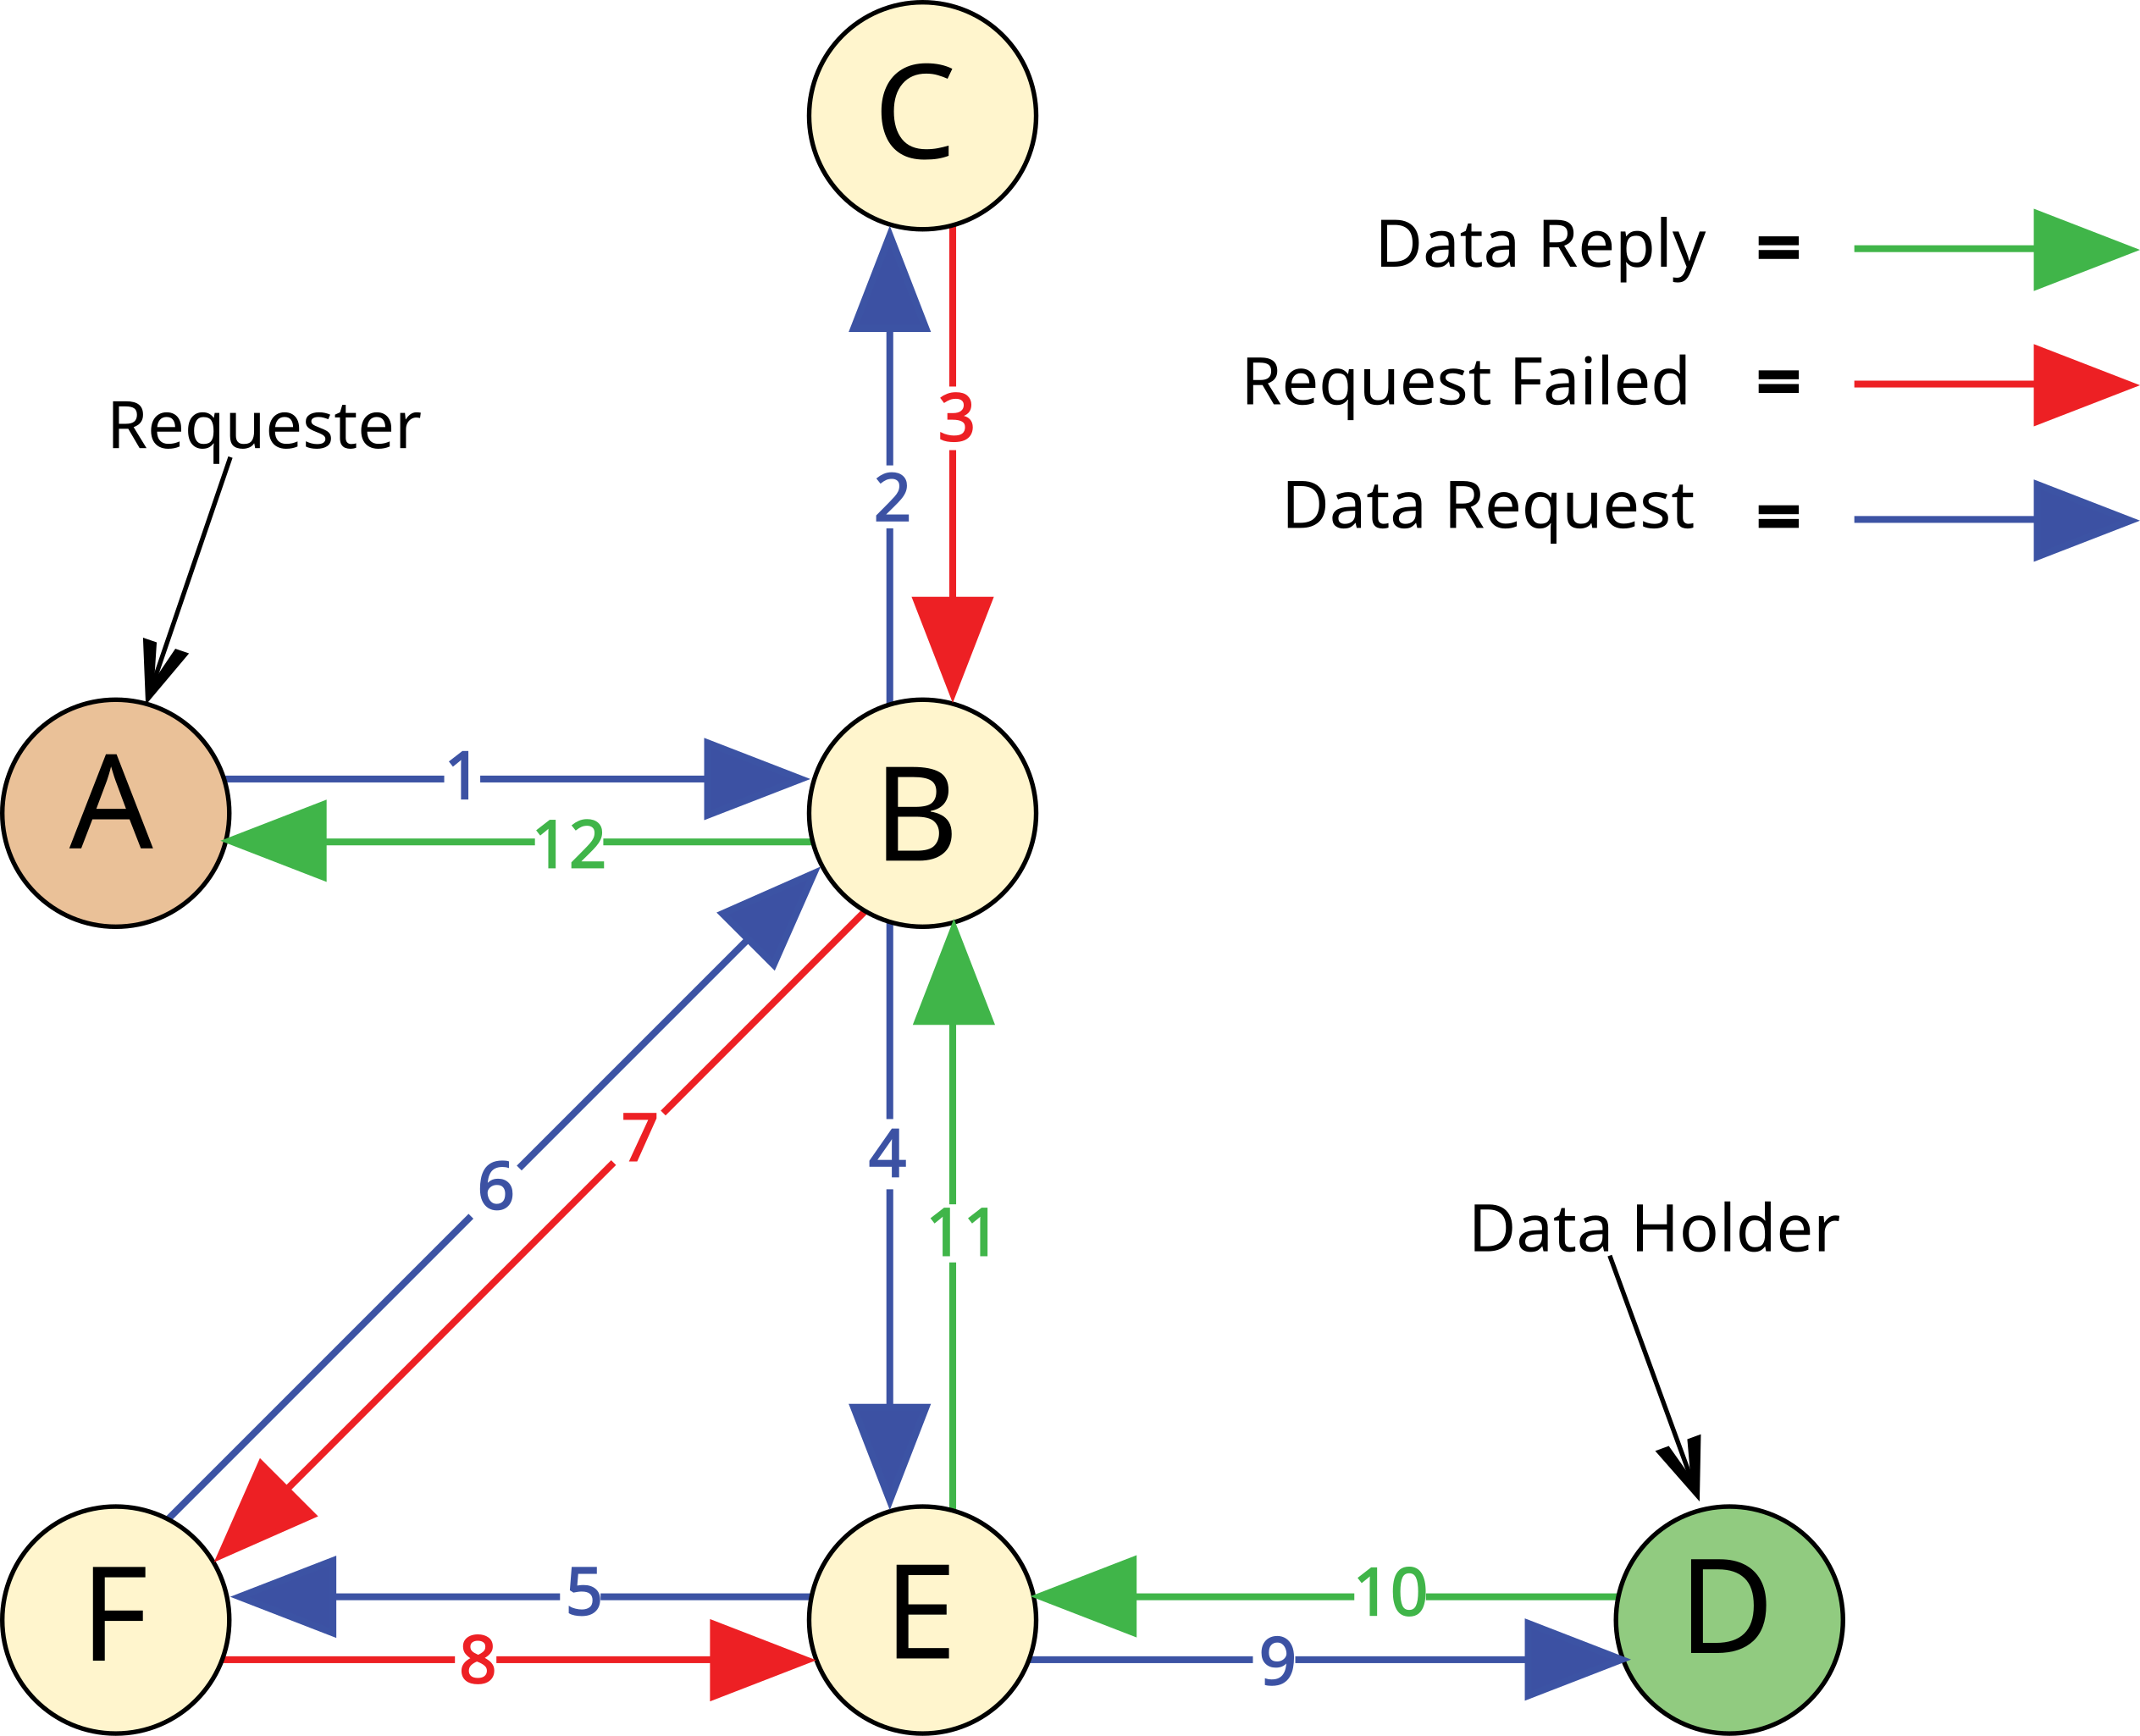
\includegraphics[width=0.75\linewidth]{Images/freenet.png}
  \caption{Request sequence in the Hyphanet (Freenet) network. By XcepticZP, Wikimedia Commons~\cite{freenet_request_sequence_zp}, licensed under CC BY-SA 3.0.}
  \label{fig:freenet_sequence}
\end{figure}

Hyphanet supports both \emph{opennet} and \emph{darknet} operating modes. In opennet, nodes automatically connect to random peers. In darknet mode, connections are established manually between trusted friends, providing additional resistance to traffic analysis and surveillance.

Routing in Hyphanet is adaptive: nodes maintain routing tables indicating which peers are most likely to have certain keys, and these tables are refined through continual use. The combination of strong encryption, distributed storage, and dynamic routing mechanisms ensures anonymity for both publishers and retrievers, while making it extremely difficult for adversaries to censor content or trace information flow within the network.

Hyphanet therefore aims to allow two or more people to share information freely, without government or other entity’s control.
At the same time, Hyphanet assumes that it is impossible to have freedom of speech without being anonymous, as it is easier to punish those who proclaim things that are not appealing to the censor rather than preventing them to do so. Hyphanet also proposed solutions to the problem of trust in the anonymous system.

The goal of Locutus \cite{locutus} is slightly different than the goal of Hyphanet; however, it shares some similarities as well. As was described before, Locutus wants to address "modern challenges", which in essence means to provide an alternative to the Internet that is known today, which is a very ambitious goal.
Ian Clarke, in his talks presenting Locutus, presents the history of the Internet along with the history of its predecessor - ARPANET. He especially emphasises the fact that ARPANET, due to the fact that it was designed in such a way that it should be resilient to potential nuclear attack, was decentralised. On the other hand, the today's Internet is not only highly centralised when it comes to the widely spread client-server architecture, but also it is mostly controlled by a few corporations that own most of the Internet services and infrastructure.

It poses a threat of data exploitation or censorship and therefore can violate individual freedom. Locutus is proposed as a solution to these problems.

It works as a shared computing platform. While Hyphanet can be compared to a shared disk, Locutus can be compared to a shared computer.

Locutus can be reached using standard web browsers as well as with an API. It proposes interesting solutions regarding many problems of today’s Internet, like users' privacy, spam, or DDoS attacks. Locutus is designed to be a platform on top of which developers can build highly interoperable, seamlessly integrated, scalable and cryptographically secured decentralised services that can be an alternative to the centralised ones that are present now.

\subsection{GNUnet}
GNUnet started in 2001 and its main goal then was to improve Freenet file sharing. The initial name for the system was GNET as GNU had not yet approved the project back then. The principle of operation was described in the paper with the same name \cite{gnet}, describing a reliable and anonymous distributed backup system. After approval a few months after the release, the project was renamed to GNUnet as it had been intended since inception. The communication mechanism in the GNET on the lowest layer was similar to SSH, although it was based on UDP, not TCP, as it did not need guarantees of proper order or packet loss and preferred to utilise lower-overhead solution. The project also described a reputation system that affected the ability of a node to interact with the network to prevent various attacks and protect the network. Instead of a global credibility system, each node had an "opinion" on other nodes that it contacted that decreased with every quest and increased for the valid replies. Queries were encrypted and hashed by the client so that the intermediaries could not decrypt the content. The hashcodes could have been combined with logical operators in order to increase searchability over systems like Freenet. Users can decide whether to use keywords of shorter length and improve usability or of longer length and increase security. The data stored on the GNET nodes were split into chunks, and each chunk was encrypted by default and stored separately with hashes as chunk identifiers. In an alternative configuration, the data can be shared in plaintext and encrypted only in transfer or, in the maximum-security configuration, XORed with a one-time pad, which results in doubling traffic/storage requirements.

The project has greatly evolved through the years, and now GNUnet is a framework for P2P networking in a decentralised and privacy-preserving manner. It aims to serve as an alternative for the traditional TCP/IP stack, creating many of the networking solutions from the ground up, addressing their major flaws from the point of view of privacy, freedom and decentralisation and at the same time providing excellent plug-in-based compatibility with existing infrastructure. As anonymity is no longer the main focus of the project, it will not be considered within the comparison.


\section{Onion routing}
While Chaum's Mix-nets provided a satisfactory level of anonymity, most of the solutions based on them introduced significant latencies and could not be used for latency-vulnerable use cases. One of the first proposals that aimed to address this issue was the ISDN-MIXes network, although it was mainly focused on the ISDN network. A different and more universal approach was PipeNet \cite{pipenet}, a protocol for low-latency anonymous communication. It was based on a network of nodes, identified by their public keys, that communicated asynchronously with each other over secure links, creating a mesh network topology. The main drawback of the network was that it assumed fully utilised links, which are expensive.

Another proposition was the UDP-based Freedom System \cite{freedom}. The primary goal of Freedom was to create a system with the strongest privacy, ease of use, and integration. Freedom used a circuit-based solution named the telescope encryption.
The solution that turned out to be the most used for low-latency anonymity communication was onion routing.

In 1995 the U.S. Naval Research Lab (NRL) researchers started working on the first prototypes of onion routing.  The first paper about the Onion Routing was released in 1996, however the final version of it was first published in 1997 and a year later, in 1998, it was published in IEEE Journal on Selected Areas in Communication \cite{onion-routing98}.

Onion routing enables anonymous connections that are highly resistant to surveillance, tracking and traffic analysis. Onion routing provides a near real-time bidirectional connection similar to the TCP socket connections. Regular Internet applications can access anonymous connections via proxies, which additionally can remove identifying information from the data stream and therefore make the communication anonymous.

It is the major difference between the Mix-net and the Onion routing as the mixes are not connection-based. It has several implications, for example onion routing does not batch the traffic and the message reordering is highly limited, which may make it more vulnerable to certain traffic analysis attacks compared to the classic Mix-nets. Nonetheless, the versatility of onion routing joined by better user experience through smaller latencies made this solution a dominant one today.
Applications that initialise communication make it through a few machines called onion routers. Onion routing was designed to be application independent, therefore a wide variety of applications could have been used. The onion routing network allows initiator and responder to have a connection between them. These connections are called anonymous socket connections, or simpler, anonymous connections. They hide who is connected to whom and why. If one wishes to go a step further and provide anonymity to the entities themselves, identifying information must be removed from the data stream before it is sent over the anonymous connection.

Basic configuration of the onion routing topology assumes that there is an onion router that sits on the firewall of the sensitive site. There is an assumption that connections within the sensitive site are protected by, for example, physical security, therefore it can also be called a secure site. Sensitive sites may be only on the initiator’s end or on both ends of the connection. Onion router at the edge of the sensitive site serves as an interface between machines within the secure site (behind the firewall) and the external network like the Internet. In order to avoid traffic analysis, the onion router sitting on the initiator’s edge should route its traffic through other onion routers within the onion network.

If both sites control onion routers then they can successfully hide their communication from eavesdroppers. On the other hand, if the responder, for example Web server, has an unprotected connection between him and the last onion router, then the data stream from the initiator must be anonymised. Otherwise analysis of the unprotected link may reveal the initiator’s identity.
Onion routers within the network are connected by permanent socket connections. Anonymous connections over the network are multiplexed over these permanent connections. For any given anonymous connection, the route in the path is precisely defined at the connection initiation, however each router in this path is only aware of the previous and the next hop in the route. The data transmitted through the onion network is modified at every onion router in order to prevent tracking of data and ensuring that compromised onion routers cannot collaborate by correlating the data stream they observe.

Onion routing’s connections by design have three phases: connection setup, data movement and connection teardown. In the first phase an initiating application establishes a socket connection to the proxy specific to an application on an onion router which intermediates its connection to the onion routing network. The proxy then determines a path through the onion network and creates a layered data structure known as an onion and sends it through the network. Each layer specifies the next hop in the route, when an onion router receives the onion it removes the layer specific to itself, identifies the next hop and forwards the remaining onion to the next onion router. According to the design each onion router should pad the onion in order to maintain a fixed size. After sending the onion, the proxy on the initiator’s site can send data through the established anonymous connection. The last onion router in the path forwards data to the proxy on the same machine, called the responder’s proxy which forwards data to the responder.
Each onion layer includes properties of the connection at each point in the path, for example cryptographic algorithms that will be used in the data movement phase or key seed material necessary for generating symmetric keys that will be used to encrypt the data sent forward (direction in which the onion travels) or backward (opposite to the onion travel’s direction) along the anonymous connection. 1999 design assumes usage of different algorithms and keys for the data that moves backwards compared to the one moving forwards. Symmetric cryptography is used for this purpose as it has significantly less computational overhead than expensive public key cryptography, therefore it is more suitable for near real-time connections.

As was mentioned, after establishing connection by sending the onion in the initialisation phase the connection is ready to perform data movement phase. Sender’s onion router will add a layer of encryption for each onion router in the path. Each onion router in the route will remove one layer of encryption and the last onion router will have a plaintext which it will pass to the receiver. For the response, the reverse order of these layers is used. Namely, the last router in the path will add the first layer of encryption and the first router will add the last one. Then the sender will receive the response encrypted with multiple layers which then he can remove in order to obtain the plaintext.

The 1999 paper describes that all information, including the onion from the initialisation phase, network control information, as well as the data that is being sent in the data movement phase, is sent in the uniform-sized cells. All cells that the onion router receives within a fixed time interval are mixed together in order to reduce correlation of the network data. For the purpose of foiling external observers, padding and bandwidth-limiting can be used. Due to the fact that each onion and each data phase cell looks different to each-onion router it is significantly harder for the attackers to perform traffic analysis.

Although the name "onion routing" may suggest that it has something to do with the third (network) layer of the ISO/OSI model, the operation logic occurs in the seventh (application) layer. It is an example of an overlay network so it refers only to the logical connections, not the physical ones. Moreover there is a significant flexibility when it comes to the protocols of the lower layers. Authors describe onion routing’s anonymous connections as protocol independent.

Onion routing turned out to be a breakthrough in the anonymous communication network field and many designs to this day implement this concept. The best known example of such a network is Tor - the most popular ACN today that will be described in a dedicated section.

Onion routing introduced an idea of reply onions, which idea is similar to Mix-nets’ reply blocks. It is the way to connect with the originator in other ways than using initial bidirectional connection with him, for example for the sake of asynchronous communication.

\subsection{Tor}

\subsubsection{History}
In the beginning of the 2000s Roger Dingledine and Paul Syverson, shortly later joined by Nick Mathewson, worked on an implementation of onion routing that could be used for everyone, not just the US Navy. It was designed to work in a decentralised network, run by people and institutions with varied interests and levels of trust. Roger Dingledine named the Tor project, which was an abbreviation for onion routing, to differentiate between other onion routing-related projects that were developed at that time.

In 2002 Tor network was deployed and its code was released under a free and open software license in order to provide more transparency to the project.

In 2004 a paper "Tor: The Second-Generation Onion Router" \cite{tor-design} was published, which described how Tor works. In the same year, the Electronic Frontier Foundation (EFF) began to fund the work on Tor.

In 2006 Tor Project Inc, a non-profit organisation was created in order to maintain development of the Tor network. Today, Tor is funded from several sources, including volunteers, foundations, and institutions.

Tor stood the test of time and turned out to be an exceptionally useful, free, and easily accessible tool against censorship, surveillance, and much more. Today, the Tor network has thousands of voluntary run relays and millions of users, and it is undoubtedly the most popular anonymous communication network in use.

\subsubsection{Modifications compared to the original onion routing design}
Tor introduces a few modifications to the original onion routing design.
Costly, slow and compromise-prone public key cryptography with long-living keys was replaced with short-living symmetric keys, achieving a perfect forward secrecy, as it will be impossible to decrypt captured traffic once the keys are deleted with the circuit teardown. Separate, dedicated proxies for every application were replaced with a universal SOCKS proxy that supports most TCP-based applications, and for the HTTP and HTTPS Tor relies on Torbutton, an add-on for Firefox, and hardened version of the Mozilla Firefox, creating a Tor Browser Bundle. The ideas of mixing, padding, and traffic shaping were rejected in favour of performance improvements and experience quality. Many TCP streams are multiplexed within a single circuit, which improves both efficiency and anonymity, as building many circuits can present a threat to anonymity, which will be discussed later. Tor proposed a leaky-pipe circuit topology, meaning that a client can communicate with all nodes in the circuit, which in theory may make traffic analysis more difficult as the data are not always going through the entire circuit. Congestion control was achieved through end-to-end acknowledgments that detect congestion. Problematic state flooding was replaced with another mechanism, directory servers; certain nodes, considered as more trusted, provide a list of known routers and their state in order for the user to be able to build a circuit. Initially, such a request was made in HTTP; however, it was later exploited by censoring regimes that were able to block the Tor network for users, and therefore the connection between the user and the directory servers started to use HTTPS. More information about the history of blocking Tor across the world will be described in a dedicated section. 
Tor nodes can advertise exit policies that describe hosts and ports to which a node is allowed to connect. End-to-end acknowledgments were introduced, enhancing security and preventing certain types of attack, for example, tagging attack. Reply onions were replaced with a more sophisticated mechanism of hidden services that allows a connection to a server whose location is not known. In order to connect with a hidden service, clients negotiate rendezvous points.

Initially Tor did not try to hide the fact that a certain user is using the network - it changed over time when regimes started to censor Tor and it was necessary to fight back - the censorship resistance became another goal of the Tor network. Today, Tor circumvents censorship with bridges that are not publicly listed relays, along with pluggable transports, a way of masking traffic.

\begin{figure}[ht]
  \centering
  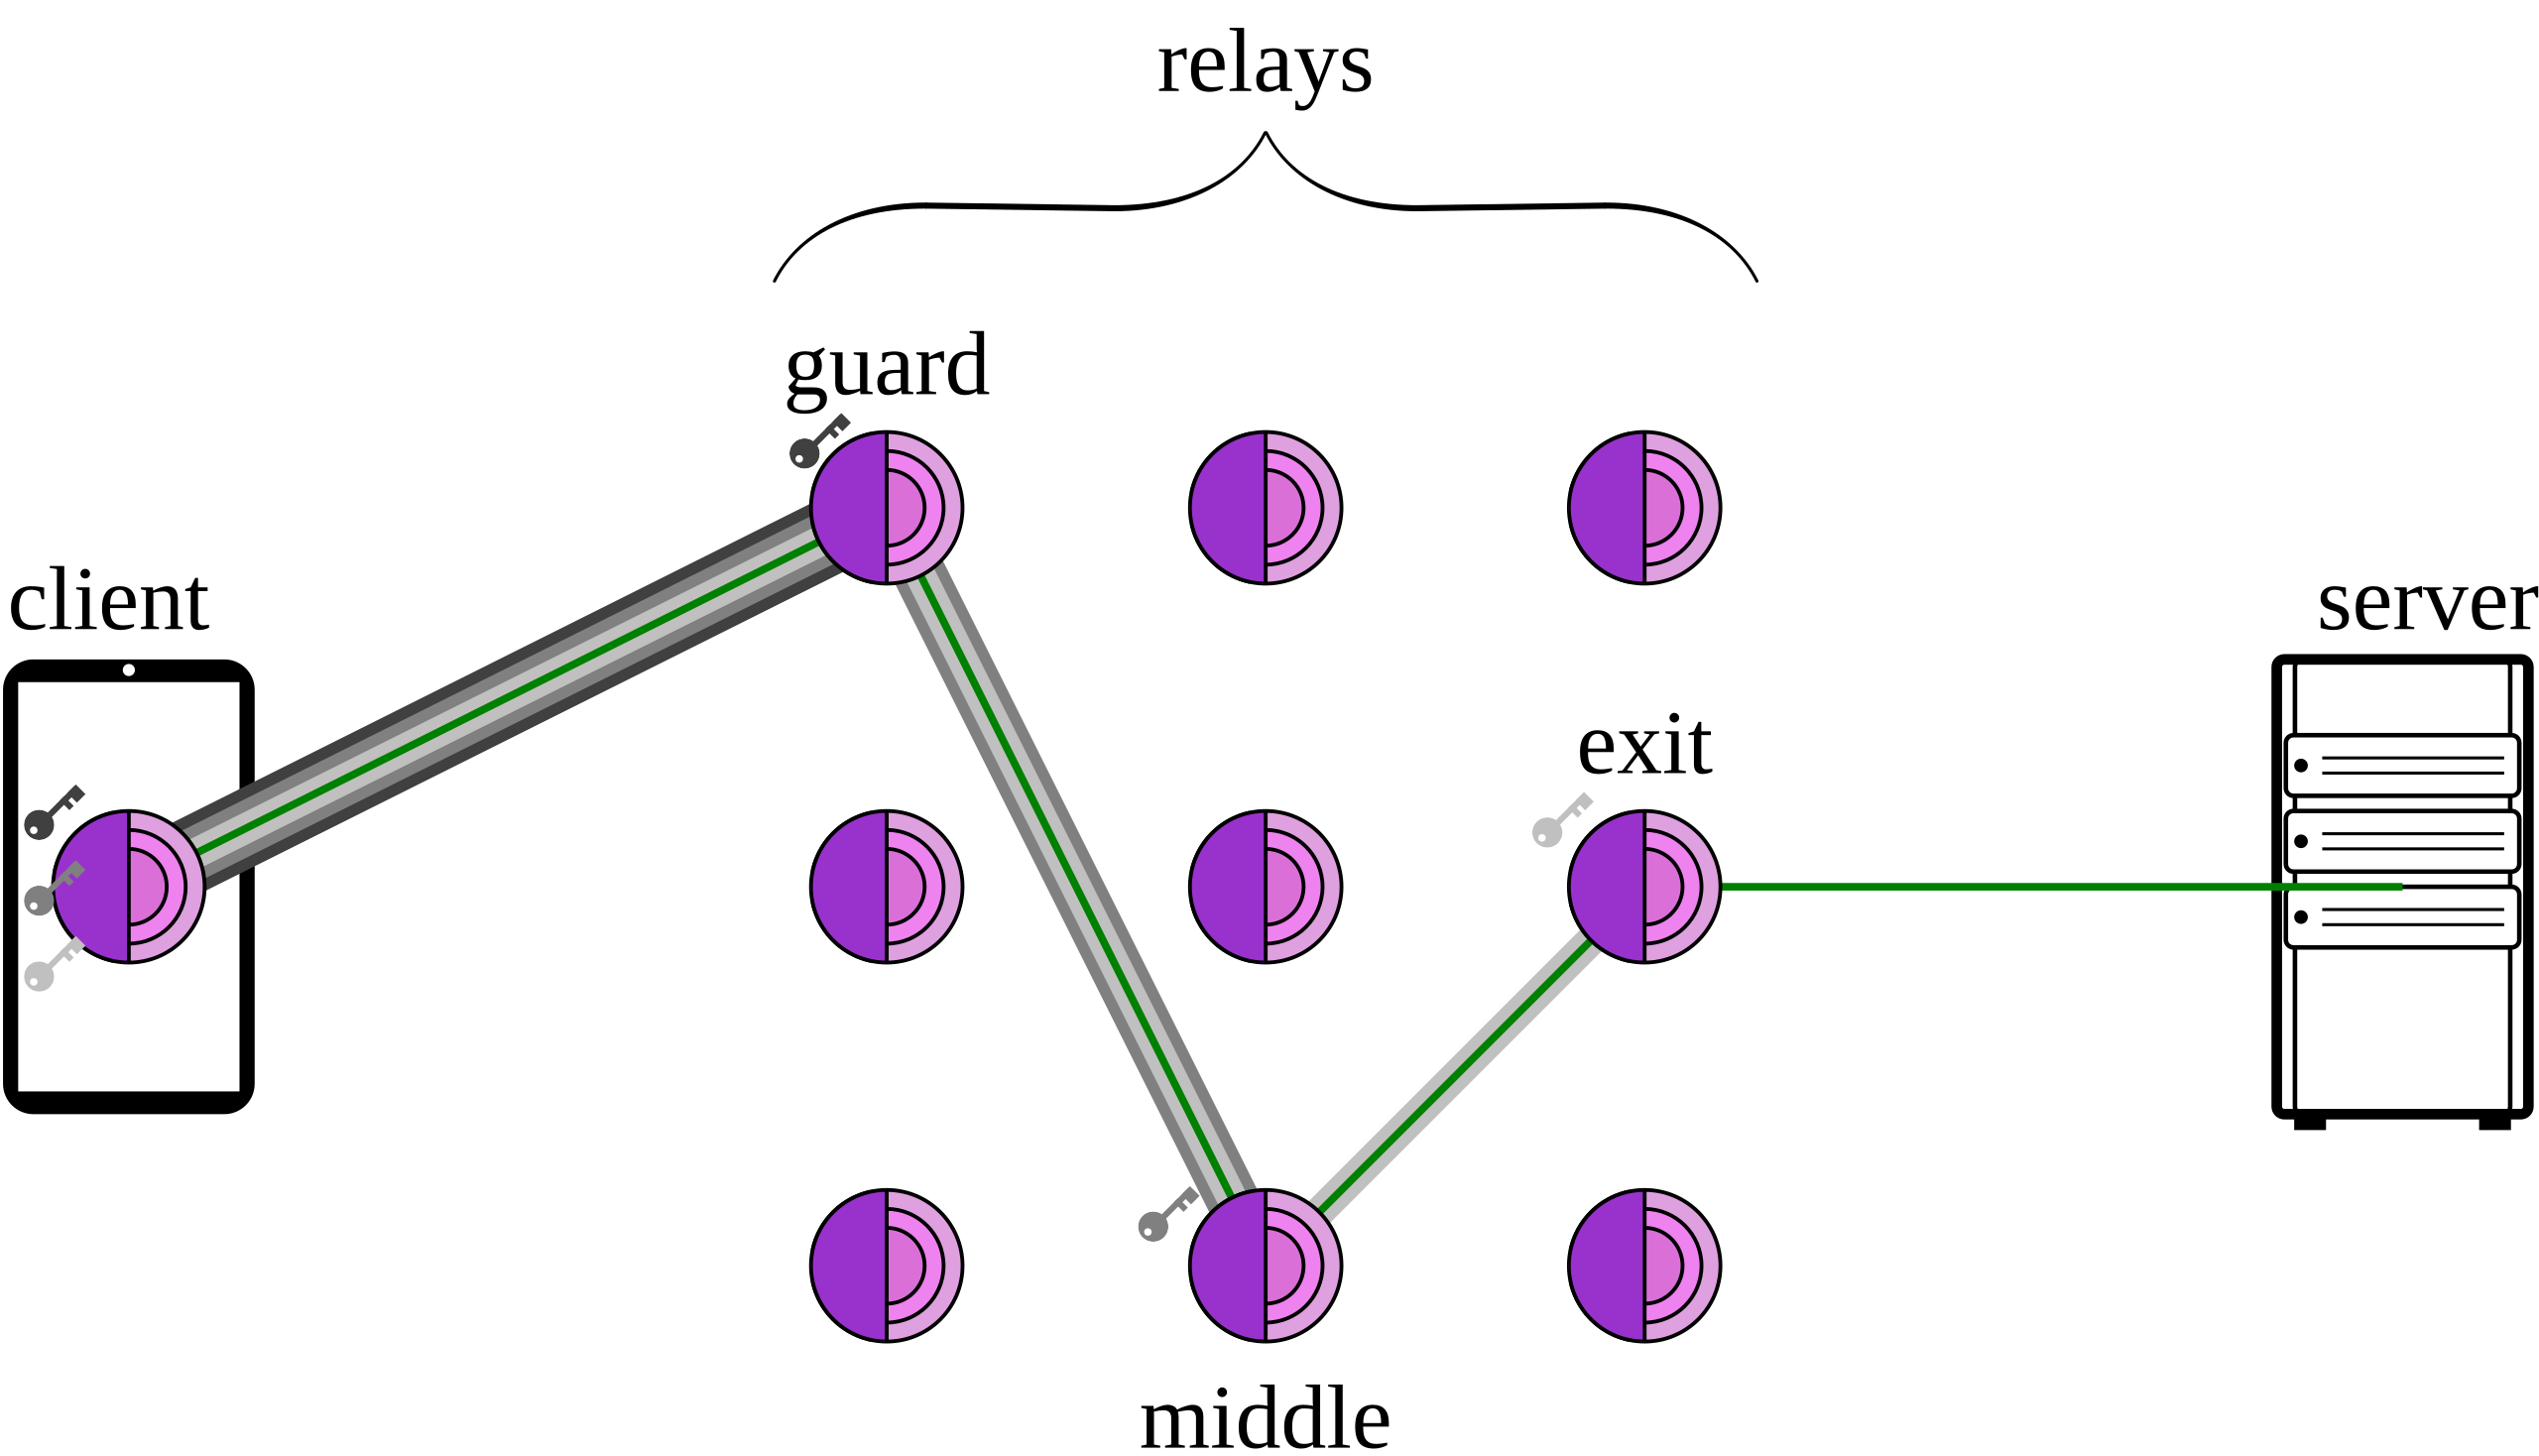
\includegraphics[width=0.75\linewidth]{Images/tor.png}
  \caption{Tor circuit diagram by Justin Tracey (Wikimedia: Tga.D), originally published in \cite{tracey_thesis}. Available on Wikimedia Commons~\cite{tracey_tor_circuit}, licensed under CC BY‑SA 4.0.}
  \label{fig:tor_circuit}
\end{figure}

The visualisation in Figure~\ref{fig:tor_circuit} illustrates onion routing using the example of Tor. The bidirectional connections between Tor nodes, as well as the link between the Tor client and the entry guard, are encrypted using symmetric cryptography of Tor; however, the link between the exit node and the destination server is not.

\subsubsection{Design and architecture overview}
Tor does not protect against a strong global passive adversary and therefore it is not secure against end-to-end traffic correlation attacks. It can protect against local passive adversaries that observe a certain fraction of a network, against generation, modification, deletion and delay of traffic or against operating or compromising some number of the onion routers. The main reason for sacrificing stronger anonymity is to achieve a compromise between anonymity, usability, and efficiency.

The project puts a great emphasis on deployability by inexpensive and easy setup, portability by supporting various operating systems, expandability for future improvements and simplicity for the sake of the ease of understanding and analysis. The main goal of these actions was to increase usability - the more people will use Tor, the larger anonymity set will be and therefore the harder it will be to identify a single user.

Tor utilises a client-server architecture. Each onion router (OR) in the onion network runs a non-root process which allows it to maintain a TLS connectivity with every onion router in the network. Users run a process called an onion proxy (OP) which allows them to establish circuits in the network, manage user connections and fetch directories. Multiple TCP streams from onion proxies are multiplexed across a single circuit. Onion routers maintain two kinds of keys: short-term onion keys and long-term identity keys. Identity keys are used for TLS certificate signatures, signing a structure called a router descriptor, which is a summary of router’s details like address, bandwidth, policies, keys et cetera. On top of that the directory servers use identity keys to sign directories. Onion keys on the other hand are used in circuit setup and symmetric ephemeral keys negotiation. TLS protocol also establishes a short-term key during onion routers’ intercommunication. Short-term keys are rotated periodically and, in order to reduce a potential key compromise impact, independently. 

Initially Tor design assumed random choosing of nodes in the circuit. This approach turned out to be problematic for various reasons. The first one was a fact that it created bottlenecks as each node had the same number of circuits as any other node and therefore the low-bandwidth ones were overloaded, the high-bandwidth ones were underutilised. The solution for this was to weight a node based on this bandwidth in a way that the high-bandwidth nodes get more circuits than the low-bandwidth ones, as well as to balance based on the node’s capabilities as the nodes that can be only the middle node would be chosen three times less frequent compared to a node that can be either entry, middle or exit node, which would also lead to bottlenecks. To prevent abuse by a potential attacker, who would advertise an impossibly high bandwidth in order to have a dangerously high probability of choosing him as a node in the circuit, Tor uses measured bandwidth instead of an advertised one. Another improvement that was made with nodes choosing was related to guard nodes. It is assumed that it is sufficient for the attacker to deanonymise user if the attacker is controlling both entry and the exit node. Considering the fact that the circuits are created rather frequently, the probability of deanonymisation in a longer period of time was exceptionally high. Guard nodes are an answer to this issue - instead of choosing three new nodes each time the circuit is created, the entry node is kept for a longer period of time. With this approach, the likelihood of deanonymisation is not increasing as rapidly with time, unless the malicious node is chosen for the guard - then the probability is even higher. Moreover, in order to decrease the likelihood of controlling both entry and exit nodes at the same time, additional diversity requirements were introduced for nodes in the circuit that prevents the creation of a circuit with two routers with the same network range or family.

\subsubsection{Cells, circuits and streams}
Tor uses fixed-size cells of 512 bytes for communication over TLS connections between onion routers and onion proxies. Cell includes the identifier of a given connection, command field that specifies a cell’s payload purpose and the payload itself. There are two kinds of cells: control cells, interpreted by the receiving node, and relay cells, responsible for end-to-end data stream. Relay cells have additional header fields compared to control cells, including: TCP stream identifier, end-to-end checksum, payload length and a specific relay command. Relay header is encrypted along with relay cell payload and decrypted along the way in the circuit.

In Tor one circuit can be shared among multiple TCP streams. Moreover, in order to avoid correlation between the Onion Proxy and the stream, a new circuit is being established periodically in the background, when the previous circuit is being used. Circuits that do not have any open streams are closed. Every minute Onion Proxy considers switching the circuit to the new one.

The Onion Proxy negotiates symmetric keys with every node in the circuit incrementally. It will first establish an encrypted connection with the first (guard) node, then through the first node with the middle relay and eventually, through the guard and the middle relay, with the third (exit) node. Establishing is done via certain cell commands and Diffie-Hellman key-exchange algorithm is utilised. It is important to mention that there is one-side entity authentication here, meaning that the Onion Proxy will know to which Onion Router it connects to, but not the other way around. Two symmetric keys are derived from each established key: one for the forward traffic and the second one for the backward one.

After establishing the circuit, relay cells can be sent. After receiving such a cell the Onion Router checks the correlated circuit and decrypts the header and payload with the session’s key. It checks the integrity of the message by verifying the digest. In order to gain computational optimisation, hash computation is often omitted and the first two bytes of the hash are zero. After verifying the message integrity it either processes the message or checks the circuit ID (circID) and OR for the next step of the circuit and replaces circID. If the exit node receives an unrecognised relay it raises an error and tears down the circuit. When Onion Proxy receives the relay response cell it unwraps the relay header and the payload with the session keys that it shares with every Onion Router in the circuit, checking the integrity with every unwrapping. 
Initial Tor TLS handshake was a straightforward mechanism that included providing supported cryptographic algorithms and parameters by the initiator and choosing them by the responder as well as providing a two-element certificate chain that proved the authenticity of the Tor node. This mechanism had to be later modified due to censoring Tor using deep packet inspection in a way that would make it appear like the usual HTTPS web traffic.
Streams utilise SOCKS protocol in order to be able to connect the Onion Proxy to the given address and port. OP either creates a new proxy or uses the newest created open circuit. From that circuit it chooses one node to be an exit node, depending on the exit policy - usually the last node.

Due to several flaws with SOCKS in the initial Tor design that could have led for example to a DNS leak, usage of privacy-aware HTTP proxies was suggested. It was later addressed by the Tor Browser bundle.

Similarly to closing TCP streams, Tor uses two-step handshake for normal closing, which is especially useful for half-closed connections, and one-step handshake for errors.

\begin{figure}[ht]
  \centering
  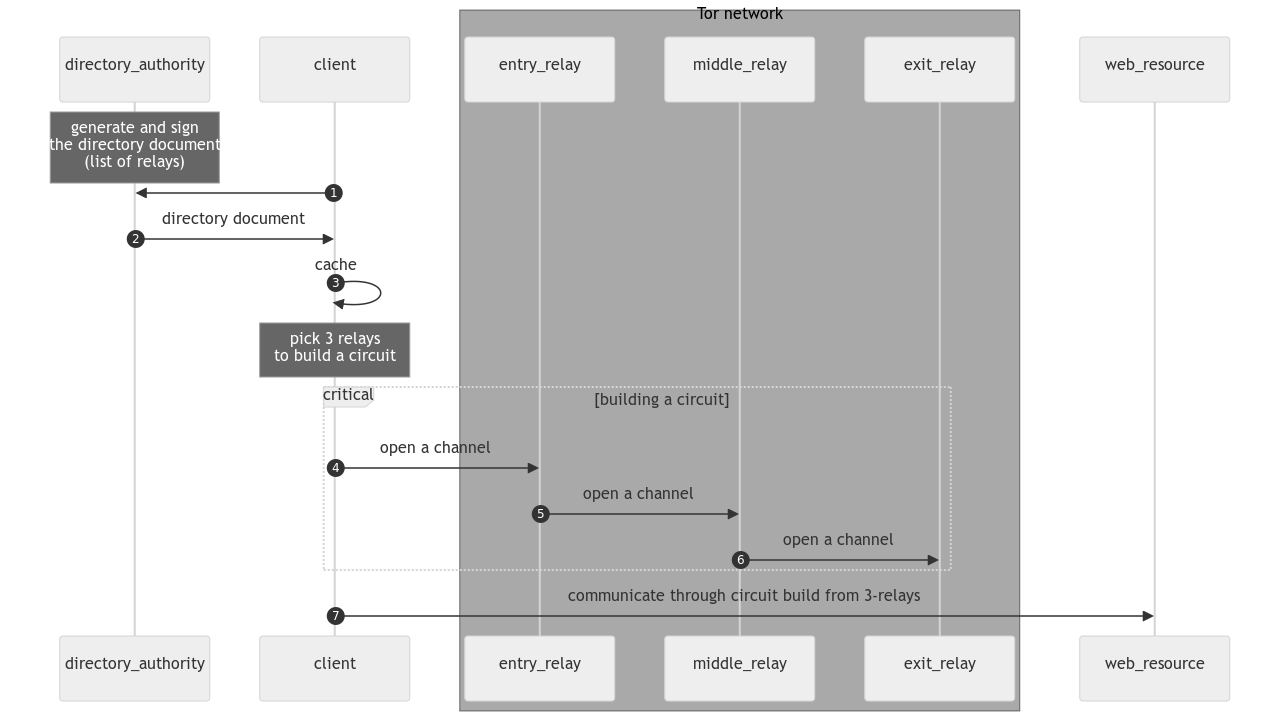
\includegraphics[width=0.8\linewidth]{Images/tor-circuit.png}
  \caption{Tor circuit setup process. Source: The Tor Project specification~\cite{torproject-specs}, licensed under CC BY 4.0.}
  \label{fig:tor_spec}
\end{figure}

Figure~\ref{fig:tor_spec} presents a sequence diagram that describes the typical circuit setup process in standard Tor usage. Initially, the user requests a signed list of relays (the directory document) from the directory servers and receives this information in response. Using the directory document, the user selects three relays to form a circuit. The circuit is then established using the telescope approach, where encrypted channels are incrementally opened through each relay, one at a time. Once the circuit is fully established, it enables secure bidirectional communication between the user and destination until the circuit teardown.

\subsubsection{QoS}
Tor includes mechanisms of QoS: congestion control, fairness and rate limiting. \textbf{Congestion control} in Tor is achieved on several levels. Firstly, it utilises TCP along with its mechanisms of congestion control and in-order guarantees. Secondly, circuit-level throttling to control the bandwidth within the circuit, where each onion router keeps a track of two windows for incoming and outgoing traffic. Thirdly, an end-to-end stream-level throttling is introduced, similar to the circuit one, however utilising a single window. To limit bandwidth usage and provide \textbf{fairness and rate limiting} Tor uses a token bucket algorithm, that helps to achieve long-term average rate of bandwidth but at the same time allowing for infrequent sudden spikes. Moreover, streams can be categorised based on the frequency of cells' appearance in order to provide a better latency for interactive streams. The risk of an end-to-end attack in this case is not an additional threat as Tor is already vulnerable to these types of attacks.

\subsubsection{Onion Services}
Tor can not only provide anonymity for the sender, which was described above, but also for the server itself (responder anonymity). It can be achieved thanks to Tor’s onion services, previously known as hidden services or location-hidden services. The server anonymity can have many benefits, which will be described in the use cases and application areas section.
The anonymous bidirectional connections is established as follows:
First the onion service creates a long-term key pair which will identify the service. Secondly, it chooses several onion routers as its introduction points (IPs), establishes a circuit with each of the IPs, providing each of them his public key, and advertises them in the lookup service which has a form of a distributed hash table - a hidden service directory (HSDir). It then signs the advertisement, otherwise known as the hidden service description, with its private key. Optionally, a part of the descriptor that includes the introduction points can be encrypted with a key that is shared between the onion service and authorised users. With this approach, the unauthorised users not only will not be able to connect to the service, but also they will be unable to discover it in the first place.
If a user wants to communicate with the onion service, looks up in the DHT for one of the introduction points of the hidden service, chooses an OR as his rendezvous point (RP), establishes a connection with both RP and IP and then announces the RP to the OS through the IP, along with a rendezvous cookie, first part of a DH handshake and optionally with additional information, encrypting everything with the onion service’s public key. Once onion service receives this message it can connect with the rendezvous point, of course through intermediate nodes, and pass the rendezvous cookie, joined by the second part of the DH handshake and a hash of the session key they are now sharing. Despite the fact that the RP connects user’s and onion service’s circuits, it is not aware of the communication between them. Neither are onion service’s IPs. Once the user sends the control cell along the circuit, the two-way anonymous communication can be performed.
Such a separation of functionalities on multiple routers provides smear-resistance, while several introduction points provide robustness and higher availability.
There is also a possibility of access control associated with optional authorisation tokens that a user can provide.
From 2015, .onion domains are recognised as special-use domains by the IESG and they can obtain TLS certificates \cite{rfc-onion-domain}. There are two companies that support issuing X.509 certificates for the .onion top level domain. First one is DigiCert, they support Extended Validation (EV) TLS certificates,  wildcards (which is an exception as EV in general do not support wildcards \cite{digicert}) and validity period up to 15 months. Second one is HARICA - they support Domain Validation (DV) certificates. While it may sound redundant as the onion services already seem to provide benefits of TLS in terms of end-to-end encryption and authentication, there can be several benefits from using TLS certificates. Firstly, mixing HTTP and HTTPS can cause sensitive information leakage \cite{harica}. Browsers enable additional security and privacy improvements when accessing HTTPS websites related to cookies and sensitive data. Moreover, certain software solutions require TLS by default and allow only the HTTPS. Additionally, users are taught to look for HTTPS when connecting to a website in order to make sure that it is a safe connection and changing their habits might be challenging. Furthermore, if the Tor client is located in a different place than the web server itself, the connection between the Tor client and web server needs to be additionally encrypted; in case of using HTTPS for the onion service the problem is solved.

Finally, an important and practical feature of onion services is that they work reliably even when the server is behind a NAT or firewall. This is possible due to the way onion services use hole punching techniques: the service initiates all outbound connections to introduction and rendezvous points, meaning it does not need to accept inbound connections directly. As a result, no port forwarding or firewall configuration is necessary, which significantly simplifies the deployment and increases accessibility for less technical users.

\subsubsection{Bridges}
Tor Bridges are Tor relays that are not publicly listed as standard nodes. They often offer additional functionalities, such as traffic obfuscation. Bridges were introduced in response to the censorship of traditional nodes or directory authorities that are easy to block due to their public availability, and the Tor project in advance planned for this. The idea was to simply encourage users from less censored parts of the world to offer themselves as private relays that will not be publicly listed for the people in censored countries.
Bridges can be distributed directly from the Tor website \cite{tor-bridges}, via e-mails from bridges@torproject.org upon request (currently it is required to send the request from a Gmail or Riseup email address) or by other means; any person can set up a bridge relay and privately share it with whom he wants.

\subsubsection{Pluggable transports}
Pluggable transports are modules that obfuscate traffic, so anyone monitoring the network activity of a user running Tor with a pluggable transport will see traffic that does not look like typical Tor usage. There are several types of pluggable transports (PTs):
\begin{enumerate}
    \item Obfsproxy
    \item Meek
    \item Snowflake
    \item WebTunnel
\end{enumerate}

\textbf{Obfsproxy} is the first pluggable transport, created in 2012, encrypts the traffic so that no specific headers are recognisable. In this case censors can either block all unrecognisable traffic, which will result in a massive number of false positive cases, or allow it, which is usually done. \textbf{Meek} is a pluggable transport created in 2014, based on domain fronting via Amazon Web Services (AWS), Microsoft Azure, or Google Cloud Platform (GCP). The basic idea behind it is to route user traffic to a cloud provider and from within the cloud reach the Tor network. \textbf{Snowflake} is yet another pluggable transport that works as a JavaScript code executed in the volunteers' browsers. The client connects to the Snowflake proxy of the volunteer through WebRTC that obfuscates his traffic, making it appear as, for example, a video call. The major advantage of this kind of pluggable transport is the simplicity of deployment without the need of dedicated software other than browser extension, although there are also dedicated standalone snowflake proxies aimed at long-term connections. The more people join as a snowflake proxy, the more difficult it will become to censor traffic without a large number of false positives. \textbf{WebTunnel}, officially announced in 2024, is a new kind of bridge that aims to circumvent censorship in heavily censored countries. Using an HTTPS proxy, similar to HTTPT \cite{httpt}. Contrary to Obfsproxy, it aims to mimic a real web server, rather than appearing as unrecognisable traffic.

\subsection{I2P}

\subsubsection{History}
The idea for I2P started in October 2001 when Lence James, known under the pseudonym 0x90, created IIP - the Invisible IRC Project as a way for instant communication with Freenet users regarding Freenet issues and for Freenet keys exchange.
In 2003 it was decided that IRC was not sufficient for the project to serve its purpose. Instead of such an approach, a universal anonymisation layer was needed for a wider variety of protocols. From then on, IIP was also referred to as InvisibleNet. 

In the same year an anonymous developer jrandom joined the project and his ambition was to expand it. He wanted to redesign the system with inspiration from Tor and Freenet projects, but at the same time many things specific to the I2P were introduced. Strong emphasis was placed on protection from organisations with enormous resources. In the same year, jrandom took control over the project, and it was renamed to the name that exists today, Invisible Internet Project, or I2P for short. Two years later, in 2005, another prominent anonymous developer joined the project - zzz, shortly after joined by yet another developer with a pseudonym Complication. In 2007 zzz with Complication took control over the project after jrandom unexpectedly quit, which caused turbulence for the project development.

Over the years, several developers joined and left the project, and many improvements were introduced. The project is to this date fully based on volunteers’ work. The project used to accept donations but they were discontinued. Today, I2P is considered one of the most popular anonymous communication networks; currently, it has around 55,000 routers, according to I2P metrics \cite{i2pmetrics, i2pmetrics2}. The number of users may be slightly larger since users from restricted countries may not act as routers.

\subsubsection{Design and architecture overview}
I2P is an overlay peer-to-peer network with full encryption and resilience against censorship, eavesdropping, and recognition. Every user, unless it is unsafe for him, contributes to the network as a router, increasing the network anonymity, creating a peer-to-peer network. Also, being a router or, in other words, participating in the I2P network is not necessarily something that should be kept as a secret, while information about connections with endpoints associated with specific applications called destinations is.

I2P utilises tunnels, encryption (both router-to-router and end-to-end), provides forward secrecy for all connections and self-authenticated network addresses.

The network consists, among others, of routers/peers communicating with each other, unidirectional tunnels (one for incoming traffic, one for outgoing traffic, contrary to the Tor bidirectional tunnels) and a distributed hash table as an internal database for information distribution. These and other elements of the I2P architecture will be described in detail in this section.

In order to connect to the I2P network, the user needs to install a Java client consisting of a static website template, email, and a BitTorrent client. As mentioned above, it also works as a router.

I2P offers a complete suite of network protocols and serves as a platform on top of which applications can be built. These applications include newsgroups, email, messaging, file sharing, web browsing, blogging, or distributed data storage.
One of the main advantages of the I2P network is its scalability. The more people use the network, the faster it is as there are more routers in the network and more traffic is being passed by them. It is also becoming more anonymous with an increasing number of users as there is much more traffic to pass with for a particular router. Due to the peer-to-peer nature, creating exit points would impose a threat of legal issues for the users, given illegal actions of some other user that would have them as the exit point. Users might not be willing to take this risk, which would definitely reduce the number of users willing to use the network. Due to this fact, along with security issues that are associated with exit points, I2P does not support exit points by default; however, it is possible to create such a proxy (outproxy) on a higher layer.

\subsubsection{Routers and destinations}
The I2P router is an entity that participates in routing the traffic of users. It has the same role as the nodes in the Tor network; however, contrary to Tor, each user that uses the I2P also routes traffic to others. Although being a router or running the I2P software is currently not a secret, it is possible that in the future, when I2P will gain more popularity and governments will try to censor it, it will become necessary to add a masking layer to circumvent the censorship. When a user first connects to the network, he connects to special-purpose routers called reseed hosts, that provide an initial set of nodes for a new router to connect with.

Destinations are cryptographic identifiers of applications within the network. The fact that a user has reached a given destination is a secret. In addition, the user who reached the destination remains anonymous.

\subsubsection{Network database}
The network database, netDb, is a distributed hash table (DHT) database based on the Kademlia algorithm that is responsible for the sharing of metadata on the network. The database is maintained by a subset of routers called floodfill routers. They are normal routers with high bandwidth, which constitute about 6\% of the network. There are two types of metadata. 

The first is \textbf{leaseSets}. It gives the instructions necessary to reach the particular destinations. LeaseSets also include a number of leases, where each lease specifies a tunnel gateway that is necessary to reach a particular destination. Lease information includes a pair of public keys for message encryption, tunnel expiration time, and recipient inbound gateway. LeaseSets are distributed through outbound tunnels to avoid correlation between leaseSets and their router and to remain the router’s identity. There is a possibility of private encrypted leaseSets for the purpose of reaching services that must not be publicly available. Such encrypted leaseSets are not published on the netDb and require appropriate decryption keys.

The second one is \textbf{routerInfo}; it gives the instructions for reaching the specific router. These instructions include a unique ID in the form of a cryptographic public key,  transport addresses and ports, timestamps, and other options that can be utilised by the user, everything digitally signed and the signature is also attached. RouterInfo is distributed by the routers directly to netDb, as this information should not be a secret.

Figure~\ref{fig:i2p_topology} illustrates the use of inbound and outbound tunnels for Alice and Bob within the I2P network. For simplicity, Charlie's inbound tunnel and Dave's outbound tunnel are omitted from the diagram. The network database contains the information necessary to allow participants to discover and reach each other's inbound tunnels.

\begin{figure}[ht]
  \centering
  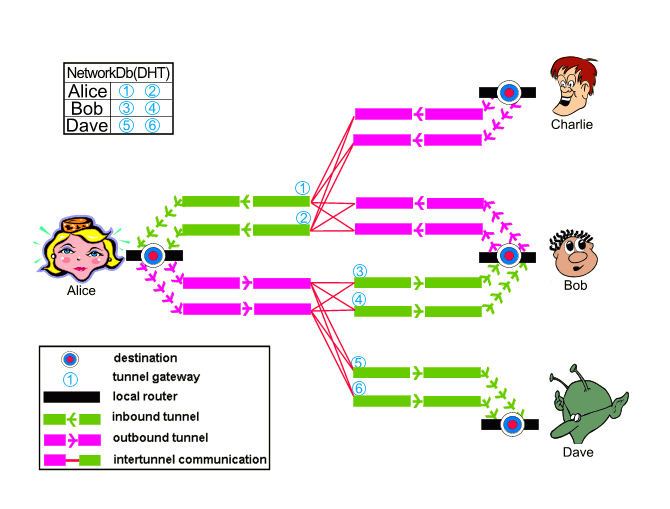
\includegraphics[width=0.75\linewidth]{Images/i2p.png}
  \caption{Simplified I2P network topology. Source: I2P documentation \cite{i2p-topology}, licensed under CC BY‑SA 4.0.}
  \label{fig:i2p-topology}
\end{figure}

\subsubsection{Tunnels and garlic routing}
A tunnel is a short-living, direct path between two points underlaid by several routers between, where layered encryption is utilised. Each router can decrypt (or "peel") the encryption layer and forward the message to the next router. The first router in the path, a tunnel starting point, is called a gateway. Tunnel ends with an endpoint. Tunnels are only one-way and for responses additional tunnel is needed. That is why there are two types of tunnels in I2P that are required for two-way communication: inbound and outbound. Inbound tunnels, as the name suggests, bring messages to the tunnel initiator and outbound tunnels send messages from the tunnel initiator. Sender’s outbound endpoint will pass the message to the recipient’s inbound gateway given appropriate instruction to forward the message. Utilising two one-way tunnels instead of one two-way tunnel makes traffic analysis harder for the adversary.

In order to build inbound and outbound tunnels a user needs to call the netDb and fetch a list of peers that can be used as hops in these tunnels. Then users can gradually, router after router, build the tunnel via construction messages. User sends the message to the first hop, then to the second hop with intermediation of the first router, then third one through first and second until the tunnel is successfully formed.
When the sender wants to send a message he first needs to find the receiver's leaseSets in the netDb in order to retrieve receiver’s inbound tunnel gateways. Sender then needs to choose one of his outbound tunnels and sends the message through this tunnel along with information to pass the message to one of the receiver’s inbound tunnel gateways. To sum up, the path of the message is as follows: first it is sent via the sender's outbound tunnel, then it is forwarded, thanks to appropriate instructions, to the receiver’s inbound tunnel.
In case the sender would like to receive a response he will need to send his destination within the message. Sender can also optionally include his leaseSets in the message so that receiver would not need to look it up in the netDb.
Despite layered encryption in tunnels that was described before, an additional end-to-end encryption needs to be used in order to protect messages that are leaving outbound tunnels and entering inbound ones. The end-to-end encryption is performed with public key cryptography.

Messages can be grouped together and form what is called a garlic. Each message in the garlic can be named a garlic clove. Garlic cloves can be accumulated in the inbound gateway and then passed via the tunnel and split in the input tunnel endpoint. That mechanism is possible due to unidirectional tunnels and would not be possible in classic, onion routing bidirectional tunnels. It is often referred to as garlic routing.
Garlic contains information about the tunnel which will be used for message sending which makes route establishment much faster.

While I2P initially proposed the introduction of batching, mixing, throttling, padding and delaying traffic, it is currently not implemented as parallel support of two types of traffic can be problematic. If it will be in the future, the network should then be considered as a hybrid solution between Mix-Nets and Onion Routing. 

Routers are chosen for the tunnel based on various metrics, including their bandwidth, capacity measured by successfully built tunnels, which is the direct indicator of their reliability, family diversity, as well as on manually adjustable individual preferences.

Figure~\ref{fig:i2p-encryption} illustrates the multiple layers of cryptography applied to messages in the I2P network, effectively providing three layers of encryption: on the link level, tunnel level, and end-to-end.

\begin{figure}[ht]
  \centering
  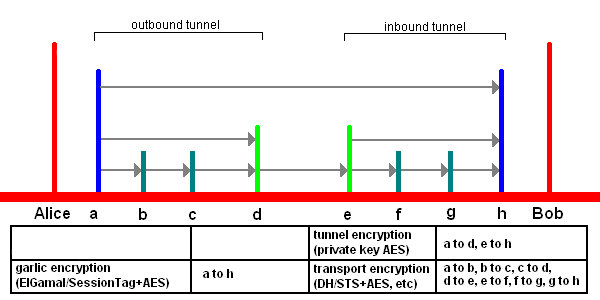
\includegraphics[width=0.75\linewidth]{Images/i2p-encryption.png}
  \caption{Message encryption in I2P. Source: I2P documentation \cite{i2p-encryption}, licensed under CC BY‑SA 4.0.}
  \label{fig:i2p-encryption}
\end{figure}

\subsubsection{I2P protocol stack}
The Invisible Internet Project proposes its protocol stack on top of which applications can be built. For analysis purposes, references to the OSI and TCP/IP stacks will be made. In theory, the TCP/IP transport layer and all lower layers are also a part of the stack; however, the overview will focus solely on the I2P-specific stack. Beginning from the bottom of I2P stack:
\begin{enumerate}
\item I2P Transport Layer
\begin{enumerate}
\item SSU2: Secure Semi-reliable UDP
\item NTCP2: NIO-based TCP
\end{enumerate}
\item I2P Tunnel Layer
\item I2P Garlic Layer
\end{enumerate}

The \textbf{I2P Transport Layer}, in the context of the TCP/IP and ISO/OSI stacks, as well as each layer after it, could be placed in the application layer. However, this specific layer can also be treated as an overlay on the traditional transport layer. This layer is responsible for providing encrypted connections between the I2P routers. These are not anonymous end-to-end connections but simple, not anonymous, hop-by-hop connections. In the I2P Transport Layer there are two protocols that are based on UDP and TCP: \textbf{SSU2} (Secure Semi-reliable UDP) and \textbf{NTCP2} (NIO-based TCP). In the future, this layer can also provide additional obfuscation that will make it harder for censors to block I2P traffic. The \textbf{I2P Tunnel Layer} is the layer that provides tunnel connections with full encryption. Protocol data units used within the I2P Tunnel Layer are tunnel messages and I2NP (I2P Network Protocol) messages. I2NP are messages used to pass information through multiple routers. Multiple I2NP messages, layered and encrypted along with instructions necessary for their delivery, are combined into a larger tunnel message which has a fixed size of 1024 bytes. Each hop in the path removes (decrypts) its layer, reads an instruction, and forwards the message to another router. The \textbf{I2P Garlic Layer} provides anonymous and encrypted end-to-end message delivery. Similarly to the tunnel layer, the I2P Garlic Layer uses I2NP messages. They are wrapped in layers to ensure anonymity for the sender as well as for the receiver. Garlic messages expand standard onion messages by allowing the message to contain multiple cloves. A clove is a fully formed message with delivery instructions.

Mentioned layers are considered as I2P core layers. There are also additional layers that are considered non-core layers:

\begin{enumerate}
\item I2P Client Layer
\item I2P End-to-End Transport Layer
\begin{enumerate}
\item Streaming library
\item Datagram library
\end{enumerate}
\item I2P Application Interface Layer
\item I2P Application Proxy Layer
\item I2P Application Layer
\end{enumerate}

The \textbf{I2P Client Layer} provides the ability to use I2P without direct router API usage. \textbf{I2CP}, or \textbf{I2P Client Protocol}, is a protocol of this layer. It provides asynchronous and secure communication by sending messages over the I2CP TCP socket between a client and a router. The \textbf{I2P End-to-End Transport Layer} provides functionalities similar to TCP and UDP from the TCP/IP transport layer, but over the I2P network. Two prominent solutions that exist within this layer are the \textbf{Streaming library} (functionality similar to TCP streams over the I2P network) and the \textbf{Datagram library} (messaging similar to UDP over the I2P network). The \textbf{I2P Application Interface Layer} provides libraries that make development on top of I2P easier. The protocols of this layer use the protocols of the \textbf{I2P End-to-End Transport Layer}. Example protocols include \textbf{SAMv3}, which supports multiple communication types, including reliable in-order TCP-like streams, UDP-like datagrams, or unauthenticated raw ones with minimal overhead. It supports many programming languages as well and can be used for creating I2P-native applications. Another example is \textbf{I2PTunnel}, which is used for creating general-purpose TCP-based connections, enabling seamless proxying of existing non-I2P applications into the I2P network without the need for writing I2P-specific code. The \textbf{I2P Application Proxy Layer} is used for proxy systems. Example protocols for this layer include SOCKS, HTTP, and IRC. Finally, the \textbf{I2P Application Layer} is a common name for the applications that can be built on top of the I2P stack.

\subsubsection{I2P applications}

There are many I2P applications, some of which are included within the standard I2P install bundle. One example of a bundled application is the \textbf{naming library and address book} - a web-of-trust-based, local naming system that allows users to add specific long I2P addresses as human-readable entries in their address book. Another included application is \textbf{I2PSnark}, a BitTorrent client that works entirely within the I2P network. While it is not the only BitTorrent client available for I2P, it is the default choice shipped with the install bundle. Typically, it is not possible to connect to non-I2P torrents from within I2P, or vice versa. Additionally, the bundle includes \textbf{I2Pmail}, also known as susimail, which is an internal and external email service operating over the I2P network.

There is also the possibility of creating custom applications and distributing them as I2P plug-ins which can then be easily integrated with I2P routers from other users. Users can access the I2P router API for example via a simple JSONRPC2 interface. 
The I2P network allows services to be hosted anonymously in the I2P network. These destinations, for example, websites, called Eepsites, are subject to the i2p pseudo-top level domain. The domain name is resolved into an I2P peer key by a proxy named EepProxy. Service providers can use solutions like I2PTunnel to share basic client-server applications in I2P, it also includes support for SOCKS proxies. On the other hand, if an application is peer-to-peer, requires a more sophisticated approach, enhanced anonymity, or performance optimisation, they can write I2P-specific code and achieve tailored solutions. There is also the possibility of embedding I2P into an application.

I2P services and applications generally work without issues, even when the user is behind a firewall or NAT. In such cases, the I2P router uses a mechanism called introducers to relay inbound connections, allowing communication without requiring open ports. However, forwarding the I2P port for both UDP and TCP can improve performance, speed, and overall integration with the network.

\subsection{Lokinet}
Lokinet is a relatively recent decentralised anonymous network that utilises onion routing architecture. The network was described in the 2018 paper \cite{loki}. It is one of the first networks that introduced economic incentives for the node runners. Lokinet introduces Low Latency Anonymous Routing Protocol (LLARP) for communication within the network. It is said to be a hybrid solution between Tor and I2P. In fact, the design is more similar to the Tor one, including client-server architecture; however, Lokinet, contrary to Tor, does not use semi-centralised directory authorities. Instead, it relies on DHT, similar to I2P, although in Lokinet DHT is built on blockchain. Moreover, LLARP is not restricted to TCP-only traffic like Tor is. Lokinet has formal support for exit nodes, similarly to Tor and contrary to I2P, which requires dedicated outproxies. Similarly to Tor and I2P, Lokinet supports services within the network - SNapps - that work analogically to Tor’s onion services or the services within I2P. Lokinet also introduces a message storage concept, for users that are temporarily offline, that is not present in Tor nor in I2P. SNapps also utilise NAT/hole punching and opening firewall ports is not necessary.

The biggest difference, however, is the placement in the ISO/OSI model; while Tor and I2P are built on top of the transport layer, Lokinet is built within the network layer and can support any IP-based protocol.

The infrastructure of Lokinet underlines a popular instant messaging app - Session, although Session is temporarily switched from utilising Lokinet directly for the sake of simplified Onion Requests due to compatibility issues on various platforms \cite{onion-requests}, however, since the infrastructure is the same, the Session user base directly increases the anonymity set of Lokinet. Moreover, the return to Lokinet is planned when the compatibility issues are solved. The return is needed as low latency properties of Lokinet will allow for anonymous voice and video calls, while the current simple Onion Requests mechanism is not able to provide such functionality.

\subsection{Other designs}
There are also newer propositions that aim to address issues with the original onion routing design or with the Tor network, as it is considered a direct successor to the onion routing design. Examples of such networks include HORNET (High-speed onion routing at the Network Layer) \cite{hornet}, TARANET (Traffic-Analysis Resistant Anonymity at the Network Layer) \cite{taranet} and Dovetail \cite{dovetail}. They introduced potential improvements in terms of latency or traffic analysis; although requiring changes in the network layer, they would be difficult to perform.

\section{Classification}

\begin{figure}[ht]
\centering
\forestset{
  default preamble={
    for tree={
      font=\sffamily,
      grow'=south,
      parent anchor=south,
      child anchor=north,
      edge={-},
      align=center,
      l sep=30pt,
      s sep=6pt,
      anchor=center,
    }
  },
  bold/.style={font=\sffamily\bfseries},
  example/.style={font=\sffamily\itshape}
}
\begin{forest}
[\textbf{anonymous communication networks}, bold
  [\textbf{single-hop proxies}, edge=dashed, bold
    [\textit{VPN services}, example]
  ]
    [\textbf{Mix-nets}, bold
      [\textbf{Loopix-based}, bold
        [\textit{Nym}, example]
      ]
    ]
    [\textbf{DC-nets}, bold]
    [\textbf{onion routing}, bold
      [\textit{Tor}, example]
      [\textit{Lokinet}, example]
      [\textbf{garlic routing}, bold
        [\textit{I2P}, example]
      ]
    ]
  [\textbf{anonymous publication systems}, bold
    [\textit{Freenet/Hyphanet}, example]
  ]
]
\end{forest}
\caption{Classification of anonymous communication networks}
\label{fig:classification}
\end{figure}

The classification of anonymous communication networks is shown in \ref{fig:classification}. The tree structure presents the main categories of ACNs that have been developed over the years, highlighting the technical diversity.

At the top of the diagram are all anonymous communication networks. The next level distinguishes five main families: anonymous publication systems, onion routing, Mix-nets, and single-hop proxies. Among these, single-hop proxies are shown with a dashed line. This is to underline that, unlike other branches, single-hop proxies do not provide anonymity by design, but only by policy. Because of this, they cannot be considered proper ACNs in the strict sense.

Anonymous publication systems (such as Freenet/Hyphanet) are also present in the classification. Although they can provide strong anonymity, their main purpose is very narrow and is strictly based on anonymous publishing and distributed, censorship-resistant storage, and they cannot serve as general-purpose universal networks. For this reason, anonymous publication systems are not included in the comparative analysis in the following chapters.

Another important family included in the classification are DC-nets. Although DC-nets have strong theoretical anonymity properties, they are not widely used in practice today due to scalability, performance limitations, and significant bandwidth overhead. However, their unique approach has inspired many later designs and improvements in the field of anonymous communication.

The other two branches represent the main technical directions in the development of the ACN. Mix-nets (and their modern descendant, Loopix-based networks such as Nym) and onion routing (including classic Tor, Lokinet, and garlic routing solutions such as I2P) are the most influential approaches, each with their own properties and typical use cases. These designs are the most important for understanding practical anonymity online today.

Because the goal of this work is to compare fully functioning and practically relevant ACNs, the following chapters focus on four representative and currently active networks: Tor, I2P, Lokinet, and Nym. These systems illustrate the main architectures and techniques found in modern anonymous communication, and the analysis will show how their design choices affect their strengths, weaknesses, and best application areas.

\section{Summary}
This chapter has presented an overview of the main technical designs, historical milestones, and representative systems in the area of anonymous communication networks. By covering everything from the earliest single-hop proxies and foundational concepts like Mix-nets, DC-nets, and onion routing, through to the systems used today such as Tor, I2P, Lokinet, and Nym, it has highlighted both the diversity and the progression of technical solutions in the field.

The technical background provided here is not just historical context; it is essential for understanding the strengths, weaknesses, and practical implications of different ACN architectures. In it is crucial for the comparative analysis carried out later in the thesis.  The following chapters build on this material directly.
